\documentclass[twoside]{book}

% Packages required by doxygen
\usepackage{calc}
\usepackage{doxygen}
\usepackage{graphicx}
\usepackage[utf8]{inputenc}
\usepackage{makeidx}
\usepackage{multicol}
\usepackage{multirow}
\usepackage{textcomp}
\usepackage[table]{xcolor}

% Font selection
\usepackage[T1]{fontenc}
\usepackage{mathptmx}
\usepackage[scaled=.90]{helvet}
\usepackage{courier}
\usepackage{amssymb}
\usepackage{sectsty}
\renewcommand{\familydefault}{\sfdefault}
\allsectionsfont{%
  \fontseries{bc}\selectfont%
  \color{darkgray}%
}
\renewcommand{\DoxyLabelFont}{%
  \fontseries{bc}\selectfont%
  \color{darkgray}%
}

% Page & text layout
\usepackage{geometry}
\geometry{%
  a4paper,%
  top=2.5cm,%
  bottom=2.5cm,%
  left=2.5cm,%
  right=2.5cm%
}
\tolerance=750
\hfuzz=15pt
\hbadness=750
\setlength{\emergencystretch}{15pt}
\setlength{\parindent}{0cm}
\setlength{\parskip}{0.2cm}
\makeatletter
\renewcommand{\paragraph}{%
  \@startsection{paragraph}{4}{0ex}{-1.0ex}{1.0ex}{%
    \normalfont\normalsize\bfseries\SS@parafont%
  }%
}
\renewcommand{\subparagraph}{%
  \@startsection{subparagraph}{5}{0ex}{-1.0ex}{1.0ex}{%
    \normalfont\normalsize\bfseries\SS@subparafont%
  }%
}
\makeatother

% Headers & footers
\usepackage{fancyhdr}
\pagestyle{fancyplain}
\fancyhead[LE]{\fancyplain{}{\bfseries\thepage}}
\fancyhead[CE]{\fancyplain{}{}}
\fancyhead[RE]{\fancyplain{}{\bfseries\leftmark}}
\fancyhead[LO]{\fancyplain{}{\bfseries\rightmark}}
\fancyhead[CO]{\fancyplain{}{}}
\fancyhead[RO]{\fancyplain{}{\bfseries\thepage}}
\fancyfoot[LE]{\fancyplain{}{}}
\fancyfoot[CE]{\fancyplain{}{}}
\fancyfoot[RE]{\fancyplain{}{\bfseries\scriptsize Generated on Mon Apr 6 2015 10\-:03\-:27 for Project Bacp\-Fse\-C by Doxygen }}
\fancyfoot[LO]{\fancyplain{}{\bfseries\scriptsize Generated on Mon Apr 6 2015 10\-:03\-:27 for Project Bacp\-Fse\-C by Doxygen }}
\fancyfoot[CO]{\fancyplain{}{}}
\fancyfoot[RO]{\fancyplain{}{}}
\renewcommand{\footrulewidth}{0.4pt}
\renewcommand{\chaptermark}[1]{%
  \markboth{#1}{}%
}
\renewcommand{\sectionmark}[1]{%
  \markright{\thesection\ #1}%
}

% Indices & bibliography
\usepackage{natbib}
\usepackage[titles]{tocloft}
\setcounter{tocdepth}{3}
\setcounter{secnumdepth}{5}
\makeindex

% Hyperlinks (required, but should be loaded last)
\usepackage{ifpdf}
\ifpdf
  \usepackage[pdftex,pagebackref=true]{hyperref}
\else
  \usepackage[ps2pdf,pagebackref=true]{hyperref}
\fi
\hypersetup{%
  colorlinks=true,%
  linkcolor=blue,%
  citecolor=blue,%
  unicode%
}

% Custom commands
\newcommand{\clearemptydoublepage}{%
  \newpage{\pagestyle{empty}\cleardoublepage}%
}


%===== C O N T E N T S =====

\begin{document}

% Titlepage & ToC
\hypersetup{pageanchor=false}
\pagenumbering{roman}
\begin{titlepage}
\vspace*{7cm}
\begin{center}%
{\Large Project Bacp\-Fse\-C }\\
\vspace*{1cm}
{\large Generated by Doxygen 1.8.6}\\
\vspace*{0.5cm}
{\small Mon Apr 6 2015 10:03:27}\\
\end{center}
\end{titlepage}
\clearemptydoublepage
\tableofcontents
\clearemptydoublepage
\pagenumbering{arabic}
\hypersetup{pageanchor=true}

%--- Begin generated contents ---
\chapter{Hierarchical Index}
\section{Class Hierarchy}
This inheritance list is sorted roughly, but not completely, alphabetically\-:\begin{DoxyCompactList}
\item \contentsline{section}{Bfc\-Prototype}{\pageref{classBfcPrototype}}{}
\begin{DoxyCompactList}
\item \contentsline{section}{Bfc\-T\-U\-I}{\pageref{classBfcTUI}}{}
\end{DoxyCompactList}
\item \contentsline{section}{Date}{\pageref{classDate}}{}
\item \contentsline{section}{State}{\pageref{classState}}{}
\item \contentsline{section}{Task}{\pageref{classTask}}{}
\item Test\-Fixture\begin{DoxyCompactList}
\item \contentsline{section}{Fixture\-Bfc\-Prototype}{\pageref{classFixtureBfcPrototype}}{}
\item \contentsline{section}{Fixture\-Bfc\-T\-U\-I}{\pageref{classFixtureBfcTUI}}{}
\item \contentsline{section}{Fixture\-Date}{\pageref{classFixtureDate}}{}
\item \contentsline{section}{Fixture\-State}{\pageref{classFixtureState}}{}
\item \contentsline{section}{Fixture\-Task}{\pageref{classFixtureTask}}{}
\end{DoxyCompactList}
\end{DoxyCompactList}

\chapter{Class Index}
\section{Class List}
Here are the classes, structs, unions and interfaces with brief descriptions\-:\begin{DoxyCompactList}
\item\contentsline{section}{\hyperlink{classBfcPrototype}{Bfc\-Prototype} \\*\hyperlink{classBfcPrototype}{Bfc\-Prototype} Class is abstract base class }{\pageref{classBfcPrototype}}{}
\item\contentsline{section}{\hyperlink{classBfcTerminal}{Bfc\-Terminal} }{\pageref{classBfcTerminal}}{}
\item\contentsline{section}{\hyperlink{classBfcTUI}{Bfc\-T\-U\-I} \\*\hyperlink{classBfcTUI}{Bfc\-T\-U\-I} Class is inherited from \hyperlink{classBfcPrototype}{Bfc\-Prototype} }{\pageref{classBfcTUI}}{}
\item\contentsline{section}{\hyperlink{classDate}{Date} \\*\hyperlink{classDate}{Date} Class is used for time recording }{\pageref{classDate}}{}
\item\contentsline{section}{\hyperlink{classFixtureBfcPrototype}{Fixture\-Bfc\-Prototype} }{\pageref{classFixtureBfcPrototype}}{}
\item\contentsline{section}{\hyperlink{classFixtureBfcTUI}{Fixture\-Bfc\-T\-U\-I} }{\pageref{classFixtureBfcTUI}}{}
\item\contentsline{section}{\hyperlink{classFixtureDate}{Fixture\-Date} }{\pageref{classFixtureDate}}{}
\item\contentsline{section}{\hyperlink{classFixtureState}{Fixture\-State} }{\pageref{classFixtureState}}{}
\item\contentsline{section}{\hyperlink{classFixtureTask}{Fixture\-Task} }{\pageref{classFixtureTask}}{}
\item\contentsline{section}{\hyperlink{classState}{State} \\*\hyperlink{classState}{State} Class is used to record a progress of a task }{\pageref{classState}}{}
\item\contentsline{section}{\hyperlink{classTask}{Task} \\*\hyperlink{classTask}{Task} Class for actual recording of tasks }{\pageref{classTask}}{}
\end{DoxyCompactList}

\chapter{File Index}
\section{File List}
Here is a list of all documented files with brief descriptions\-:\begin{DoxyCompactList}
\item\contentsline{section}{\hyperlink{BfcPrototype_8cc}{Bfc\-Prototype.\-cc} \\*Implementation for \hyperlink{classBfcPrototype}{Bfc\-Prototype} Class }{\pageref{BfcPrototype_8cc}}{}
\item\contentsline{section}{\hyperlink{BfcPrototype_8h}{Bfc\-Prototype.\-h} \\*Header file of \hyperlink{classBfcPrototype}{Bfc\-Prototype} Class }{\pageref{BfcPrototype_8h}}{}
\item\contentsline{section}{\hyperlink{BfcTUI_8cc}{Bfc\-T\-U\-I.\-cc} \\*Implementation for \hyperlink{classBfcTUI}{Bfc\-T\-U\-I} Class }{\pageref{BfcTUI_8cc}}{}
\item\contentsline{section}{\hyperlink{BfcTUI_8h}{Bfc\-T\-U\-I.\-h} \\*Header file of \hyperlink{classBfcTUI}{Bfc\-T\-U\-I} inherited from \hyperlink{classBfcPrototype}{Bfc\-Prototype} }{\pageref{BfcTUI_8h}}{}
\item\contentsline{section}{\hyperlink{Date_8cc}{Date.\-cc} \\*Implementation of \hyperlink{classDate}{Date} Class }{\pageref{Date_8cc}}{}
\item\contentsline{section}{\hyperlink{Date_8h}{Date.\-h} \\*Header file of \hyperlink{classDate}{Date} Class }{\pageref{Date_8h}}{}
\item\contentsline{section}{\hyperlink{FixtureBfcPrototype_8h}{Fixture\-Bfc\-Prototype.\-h} \\*Cpp\-Unit Fixture setup for \hyperlink{classBfcPrototype}{Bfc\-Prototype} class }{\pageref{FixtureBfcPrototype_8h}}{}
\item\contentsline{section}{\hyperlink{FixtureBfcTUI_8h}{Fixture\-Bfc\-T\-U\-I.\-h} \\*Cpp\-Unit Fixture setup for \hyperlink{classBfcTUI}{Bfc\-T\-U\-I} class }{\pageref{FixtureBfcTUI_8h}}{}
\item\contentsline{section}{\hyperlink{FixtureDate_8h}{Fixture\-Date.\-h} \\*Cpp\-Unit Fixture setup for \hyperlink{classDate}{Date} class }{\pageref{FixtureDate_8h}}{}
\item\contentsline{section}{\hyperlink{FixtureState_8h}{Fixture\-State.\-h} \\*Cpp\-Unit Fixture setup for \hyperlink{classState}{State} class }{\pageref{FixtureState_8h}}{}
\item\contentsline{section}{\hyperlink{FixtureTask_8h}{Fixture\-Task.\-h} \\*Cpp\-Unit Fixture setup for \hyperlink{classTask}{Task} class }{\pageref{FixtureTask_8h}}{}
\item\contentsline{section}{\hyperlink{State_8cc}{State.\-cc} \\*Implementation of \hyperlink{classState}{State} Class }{\pageref{State_8cc}}{}
\item\contentsline{section}{\hyperlink{State_8h}{State.\-h} \\*Header file of \hyperlink{classState}{State} Class }{\pageref{State_8h}}{}
\item\contentsline{section}{\hyperlink{Task_8cc}{Task.\-cc} \\*Implementation for \hyperlink{classTask}{Task} Class }{\pageref{Task_8cc}}{}
\item\contentsline{section}{\hyperlink{Task_8h}{Task.\-h} \\*Header file of \hyperlink{classTask}{Task} Class }{\pageref{Task_8h}}{}
\item\contentsline{section}{\hyperlink{TestDate_8cc}{Test\-Date.\-cc} \\*Test program for \hyperlink{classDate}{Date} Class }{\pageref{TestDate_8cc}}{}
\item\contentsline{section}{\hyperlink{TestState_8cc}{Test\-State.\-cc} \\*Test program for \hyperlink{classState}{State} Class }{\pageref{TestState_8cc}}{}
\item\contentsline{section}{\hyperlink{TestTask_8cc}{Test\-Task.\-cc} \\*Test program for \hyperlink{classTask}{Task} Class }{\pageref{TestTask_8cc}}{}
\end{DoxyCompactList}

\chapter{Class Documentation}
\hypertarget{classBfcPrototype}{\section{Bfc\-Prototype Class Reference}
\label{classBfcPrototype}\index{Bfc\-Prototype@{Bfc\-Prototype}}
}


\hyperlink{classBfcPrototype}{Bfc\-Prototype} Class is abstract base class.  




{\ttfamily \#include $<$Bfc\-Prototype.\-h$>$}

Inheritance diagram for Bfc\-Prototype\-:\begin{figure}[H]
\begin{center}
\leavevmode
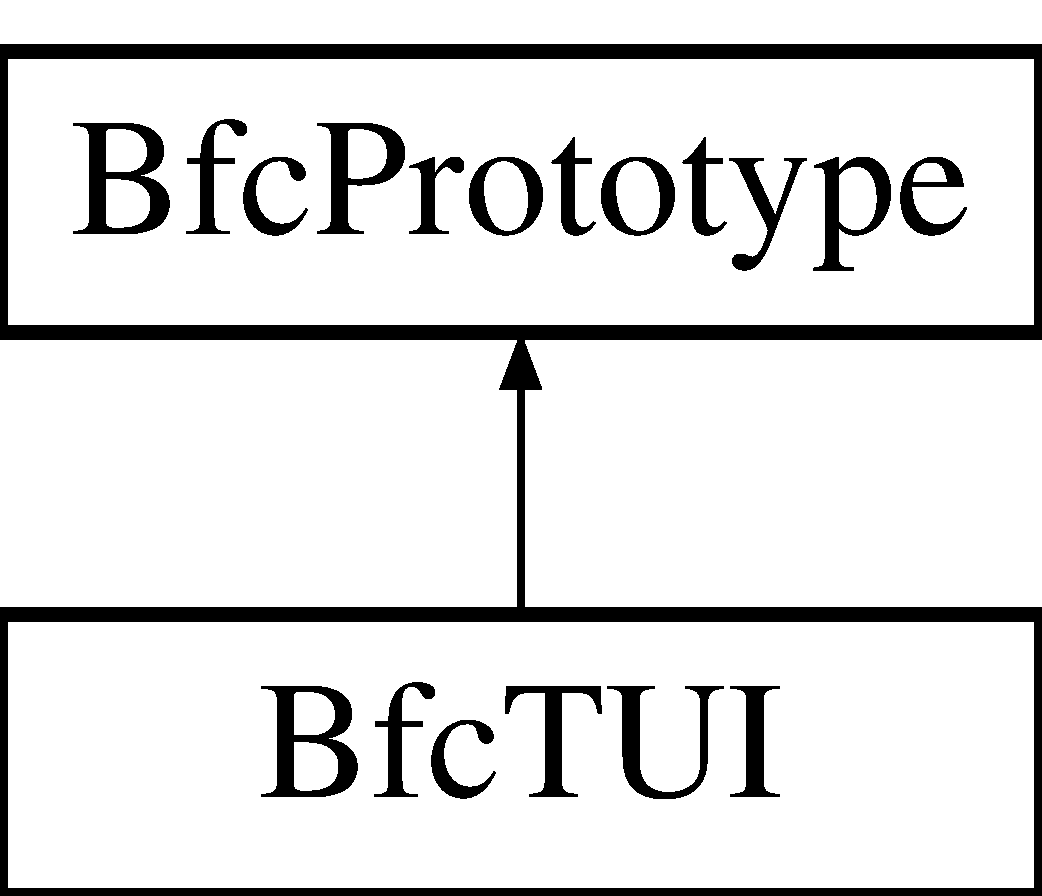
\includegraphics[height=3.000000cm]{classBfcPrototype}
\end{center}
\end{figure}
\subsection*{Public Member Functions}
\begin{DoxyCompactItemize}
\item 
\hyperlink{classBfcPrototype_a1d7d4392c17131eec1bc4219c2570433}{Bfc\-Prototype} ()
\item 
\hyperlink{classBfcPrototype_a004df1fc2cc7e03a4263edbe58c8f9fd}{$\sim$\-Bfc\-Prototype} ()
\item 
const int \hyperlink{classBfcPrototype_a1406e452c20ef38bca9067fefee33131}{get\-Max\-Task\-In\-Progress} ()
\item 
void \hyperlink{classBfcPrototype_ac38bd69cfe25044d2d866f2418795095}{set\-Record\-Loaded} (bool rl)
\item 
bool \hyperlink{classBfcPrototype_ad043f4e365502a6aec354d4f628c1404}{get\-Record\-Loaded} ()
\item 
void \hyperlink{classBfcPrototype_abb4cd3d18d2646878e00f910a89def2d}{set\-Start\-Date} (const \hyperlink{classDate}{Date} \&sd)
\item 
\hyperlink{classDate}{Date} \hyperlink{classBfcPrototype_affedd6397fcaef70f5fa397abbbf2901}{get\-Start\-Date} ()
\item 
void \hyperlink{classBfcPrototype_ab0c5d38d1e9cf0fe02e3fb5da830a802}{set\-End\-Date} (const \hyperlink{classDate}{Date} \&ed)
\item 
\hyperlink{classDate}{Date} \hyperlink{classBfcPrototype_ace745963c4c4fca8cae7c26240acf896}{get\-End\-Date} ()
\item 
void \hyperlink{classBfcPrototype_a063443b1a0a90b795c156381b41e915d}{set\-Num\-Of\-Task\-Uncomplete} (int ntu)
\item 
int \hyperlink{classBfcPrototype_af9a1299268eefad25f59b7bdb7dba5d7}{get\-Num\-Of\-Task\-Uncomplete} ()
\item 
void \hyperlink{classBfcPrototype_a3ac9f7f398cfdf3cc499f955f263672f}{set\-Num\-Of\-Task\-Cancelled} (int ntc)
\item 
int \hyperlink{classBfcPrototype_ae24a6187235106026e978fcbe49c1944}{get\-Num\-Of\-Task\-Cancelled} ()
\item 
std\-::vector$<$ \hyperlink{classTask}{Task} $>$ \& \hyperlink{classBfcPrototype_a414637b5643f0ef2a8834d1d591da364}{get\-Tasks} ()
\item 
virtual void \hyperlink{classBfcPrototype_a5dc018641f00dd03d166a6df7dcfbc4a}{read\-States} (std\-::istream \&is, \hyperlink{classTask}{Task} \&bk)
\item 
virtual void \hyperlink{classBfcPrototype_a664d219b93aa7ecf98b2686c72f918f6}{read\-Tasks} (std\-::istream \&is, std\-::vector$<$ \hyperlink{classTask}{Task} $>$ \&ts)
\item 
virtual void \hyperlink{classBfcPrototype_aa678371c41f50fe28619a589f41bb6dc}{run} ()
\end{DoxyCompactItemize}
\subsection*{Protected Member Functions}
\begin{DoxyCompactItemize}
\item 
void \hyperlink{classBfcPrototype_a8708a39c0aba8aa6d2987c17ec282f7b}{init} ()
\end{DoxyCompactItemize}
\subsection*{Private Attributes}
\begin{DoxyCompactItemize}
\item 
const int \hyperlink{classBfcPrototype_a9549b48b56475a2f2a1bded3f3ac09a4}{max\-Task\-In\-Progress} = 15
\item 
bool \hyperlink{classBfcPrototype_ac719ad28f80b4c8955ba516ac68471cc}{record\-Loaded}
\item 
\hyperlink{classDate}{Date} \hyperlink{classBfcPrototype_a636fde08f1c5518862f9d2603f73ebae}{start\-Date}
\item 
\hyperlink{classDate}{Date} \hyperlink{classBfcPrototype_a88db45d376d68c919a7a43e92adf4e23}{end\-Date}
\item 
int \hyperlink{classBfcPrototype_ab506fb074e721612c0838e2c37c93e09}{num\-Of\-Task\-Uncomplete}
\item 
int \hyperlink{classBfcPrototype_a1b1f3d0e3410f241e63884c11e36451a}{num\-Of\-Task\-Cancelled}
\item 
std\-::vector$<$ \hyperlink{classTask}{Task} $>$ \hyperlink{classBfcPrototype_a2724416668b0a82b442df12f90360e95}{tasks}
\end{DoxyCompactItemize}


\subsection{Detailed Description}
\hyperlink{classBfcPrototype}{Bfc\-Prototype} Class is abstract base class. 

\hyperlink{classBfcPrototype}{Bfc\-Prototype} Class serves as the abstract base class for variety Bacpfsec\-T\-U\-I and Bacpfsec\-G\-U\-I would inherited from \hyperlink{classBfcPrototype}{Bfc\-Prototype} 

\subsection{Constructor \& Destructor Documentation}
\hypertarget{classBfcPrototype_a1d7d4392c17131eec1bc4219c2570433}{\index{Bfc\-Prototype@{Bfc\-Prototype}!Bfc\-Prototype@{Bfc\-Prototype}}
\index{Bfc\-Prototype@{Bfc\-Prototype}!BfcPrototype@{Bfc\-Prototype}}
\subsubsection[{Bfc\-Prototype}]{\setlength{\rightskip}{0pt plus 5cm}Bfc\-Prototype\-::\-Bfc\-Prototype (
\begin{DoxyParamCaption}
{}
\end{DoxyParamCaption}
)}}\label{classBfcPrototype_a1d7d4392c17131eec1bc4219c2570433}
Default constructor \hypertarget{classBfcPrototype_a004df1fc2cc7e03a4263edbe58c8f9fd}{\index{Bfc\-Prototype@{Bfc\-Prototype}!$\sim$\-Bfc\-Prototype@{$\sim$\-Bfc\-Prototype}}
\index{$\sim$\-Bfc\-Prototype@{$\sim$\-Bfc\-Prototype}!BfcPrototype@{Bfc\-Prototype}}
\subsubsection[{$\sim$\-Bfc\-Prototype}]{\setlength{\rightskip}{0pt plus 5cm}Bfc\-Prototype\-::$\sim$\-Bfc\-Prototype (
\begin{DoxyParamCaption}
{}
\end{DoxyParamCaption}
)}}\label{classBfcPrototype_a004df1fc2cc7e03a4263edbe58c8f9fd}
Destructor 

\subsection{Member Function Documentation}
\hypertarget{classBfcPrototype_ace745963c4c4fca8cae7c26240acf896}{\index{Bfc\-Prototype@{Bfc\-Prototype}!get\-End\-Date@{get\-End\-Date}}
\index{get\-End\-Date@{get\-End\-Date}!BfcPrototype@{Bfc\-Prototype}}
\subsubsection[{get\-End\-Date}]{\setlength{\rightskip}{0pt plus 5cm}{\bf Date} Bfc\-Prototype\-::get\-End\-Date (
\begin{DoxyParamCaption}
{}
\end{DoxyParamCaption}
)}}\label{classBfcPrototype_ace745963c4c4fca8cae7c26240acf896}
Getter for end\-Date \hypertarget{classBfcPrototype_a1406e452c20ef38bca9067fefee33131}{\index{Bfc\-Prototype@{Bfc\-Prototype}!get\-Max\-Task\-In\-Progress@{get\-Max\-Task\-In\-Progress}}
\index{get\-Max\-Task\-In\-Progress@{get\-Max\-Task\-In\-Progress}!BfcPrototype@{Bfc\-Prototype}}
\subsubsection[{get\-Max\-Task\-In\-Progress}]{\setlength{\rightskip}{0pt plus 5cm}const int Bfc\-Prototype\-::get\-Max\-Task\-In\-Progress (
\begin{DoxyParamCaption}
{}
\end{DoxyParamCaption}
)}}\label{classBfcPrototype_a1406e452c20ef38bca9067fefee33131}
Getter for max\-Task\-In\-Progress \hypertarget{classBfcPrototype_ae24a6187235106026e978fcbe49c1944}{\index{Bfc\-Prototype@{Bfc\-Prototype}!get\-Num\-Of\-Task\-Cancelled@{get\-Num\-Of\-Task\-Cancelled}}
\index{get\-Num\-Of\-Task\-Cancelled@{get\-Num\-Of\-Task\-Cancelled}!BfcPrototype@{Bfc\-Prototype}}
\subsubsection[{get\-Num\-Of\-Task\-Cancelled}]{\setlength{\rightskip}{0pt plus 5cm}int Bfc\-Prototype\-::get\-Num\-Of\-Task\-Cancelled (
\begin{DoxyParamCaption}
{}
\end{DoxyParamCaption}
)}}\label{classBfcPrototype_ae24a6187235106026e978fcbe49c1944}
Getter for num\-Of\-Task\-Cancelled \hypertarget{classBfcPrototype_af9a1299268eefad25f59b7bdb7dba5d7}{\index{Bfc\-Prototype@{Bfc\-Prototype}!get\-Num\-Of\-Task\-Uncomplete@{get\-Num\-Of\-Task\-Uncomplete}}
\index{get\-Num\-Of\-Task\-Uncomplete@{get\-Num\-Of\-Task\-Uncomplete}!BfcPrototype@{Bfc\-Prototype}}
\subsubsection[{get\-Num\-Of\-Task\-Uncomplete}]{\setlength{\rightskip}{0pt plus 5cm}int Bfc\-Prototype\-::get\-Num\-Of\-Task\-Uncomplete (
\begin{DoxyParamCaption}
{}
\end{DoxyParamCaption}
)}}\label{classBfcPrototype_af9a1299268eefad25f59b7bdb7dba5d7}
Getter for num\-Of\-Task\-Uncomplete \hypertarget{classBfcPrototype_ad043f4e365502a6aec354d4f628c1404}{\index{Bfc\-Prototype@{Bfc\-Prototype}!get\-Record\-Loaded@{get\-Record\-Loaded}}
\index{get\-Record\-Loaded@{get\-Record\-Loaded}!BfcPrototype@{Bfc\-Prototype}}
\subsubsection[{get\-Record\-Loaded}]{\setlength{\rightskip}{0pt plus 5cm}bool Bfc\-Prototype\-::get\-Record\-Loaded (
\begin{DoxyParamCaption}
{}
\end{DoxyParamCaption}
)}}\label{classBfcPrototype_ad043f4e365502a6aec354d4f628c1404}
Getter for record\-Loaded \hypertarget{classBfcPrototype_affedd6397fcaef70f5fa397abbbf2901}{\index{Bfc\-Prototype@{Bfc\-Prototype}!get\-Start\-Date@{get\-Start\-Date}}
\index{get\-Start\-Date@{get\-Start\-Date}!BfcPrototype@{Bfc\-Prototype}}
\subsubsection[{get\-Start\-Date}]{\setlength{\rightskip}{0pt plus 5cm}{\bf Date} Bfc\-Prototype\-::get\-Start\-Date (
\begin{DoxyParamCaption}
{}
\end{DoxyParamCaption}
)}}\label{classBfcPrototype_affedd6397fcaef70f5fa397abbbf2901}
Getter for start\-Date \hypertarget{classBfcPrototype_a414637b5643f0ef2a8834d1d591da364}{\index{Bfc\-Prototype@{Bfc\-Prototype}!get\-Tasks@{get\-Tasks}}
\index{get\-Tasks@{get\-Tasks}!BfcPrototype@{Bfc\-Prototype}}
\subsubsection[{get\-Tasks}]{\setlength{\rightskip}{0pt plus 5cm}std\-::vector$<$ {\bf Task} $>$ \& Bfc\-Prototype\-::get\-Tasks (
\begin{DoxyParamCaption}
{}
\end{DoxyParamCaption}
)}}\label{classBfcPrototype_a414637b5643f0ef2a8834d1d591da364}
Reference getter for vector tasks \hypertarget{classBfcPrototype_a8708a39c0aba8aa6d2987c17ec282f7b}{\index{Bfc\-Prototype@{Bfc\-Prototype}!init@{init}}
\index{init@{init}!BfcPrototype@{Bfc\-Prototype}}
\subsubsection[{init}]{\setlength{\rightskip}{0pt plus 5cm}void Bfc\-Prototype\-::init (
\begin{DoxyParamCaption}
{}
\end{DoxyParamCaption}
)\hspace{0.3cm}{\ttfamily [protected]}}}\label{classBfcPrototype_a8708a39c0aba8aa6d2987c17ec282f7b}
Protected initializer

Helper to initialize all the private member \hypertarget{classBfcPrototype_a5dc018641f00dd03d166a6df7dcfbc4a}{\index{Bfc\-Prototype@{Bfc\-Prototype}!read\-States@{read\-States}}
\index{read\-States@{read\-States}!BfcPrototype@{Bfc\-Prototype}}
\subsubsection[{read\-States}]{\setlength{\rightskip}{0pt plus 5cm}void Bfc\-Prototype\-::read\-States (
\begin{DoxyParamCaption}
\item[{std\-::istream \&}]{is, }
\item[{{\bf Task} \&}]{bk}
\end{DoxyParamCaption}
)\hspace{0.3cm}{\ttfamily [virtual]}}}\label{classBfcPrototype_a5dc018641f00dd03d166a6df7dcfbc4a}
Virtual \hyperlink{classBfcPrototype_a5dc018641f00dd03d166a6df7dcfbc4a}{read\-States()}

Get the record from stream and update the task and private members \hypertarget{classBfcPrototype_a664d219b93aa7ecf98b2686c72f918f6}{\index{Bfc\-Prototype@{Bfc\-Prototype}!read\-Tasks@{read\-Tasks}}
\index{read\-Tasks@{read\-Tasks}!BfcPrototype@{Bfc\-Prototype}}
\subsubsection[{read\-Tasks}]{\setlength{\rightskip}{0pt plus 5cm}void Bfc\-Prototype\-::read\-Tasks (
\begin{DoxyParamCaption}
\item[{std\-::istream \&}]{is, }
\item[{std\-::vector$<$ {\bf Task} $>$ \&}]{ts}
\end{DoxyParamCaption}
)\hspace{0.3cm}{\ttfamily [virtual]}}}\label{classBfcPrototype_a664d219b93aa7ecf98b2686c72f918f6}
Virtual \hyperlink{classBfcPrototype_a664d219b93aa7ecf98b2686c72f918f6}{read\-Tasks()}

Get the record from stream and update the tasks and private members \hypertarget{classBfcPrototype_aa678371c41f50fe28619a589f41bb6dc}{\index{Bfc\-Prototype@{Bfc\-Prototype}!run@{run}}
\index{run@{run}!BfcPrototype@{Bfc\-Prototype}}
\subsubsection[{run}]{\setlength{\rightskip}{0pt plus 5cm}void Bfc\-Prototype\-::run (
\begin{DoxyParamCaption}
{}
\end{DoxyParamCaption}
)\hspace{0.3cm}{\ttfamily [virtual]}}}\label{classBfcPrototype_aa678371c41f50fe28619a589f41bb6dc}
Virtual \hyperlink{classBfcPrototype_aa678371c41f50fe28619a589f41bb6dc}{run()}

Implemented through inheritence 

Reimplemented in \hyperlink{classBfcTUI_a3cbe28345432cfc02537f879be1b2395}{Bfc\-T\-U\-I}, and \hyperlink{classBfcTerminal_afcd4a80a531b32527c058cf3c341a9b7}{Bfc\-Terminal}.

\hypertarget{classBfcPrototype_ab0c5d38d1e9cf0fe02e3fb5da830a802}{\index{Bfc\-Prototype@{Bfc\-Prototype}!set\-End\-Date@{set\-End\-Date}}
\index{set\-End\-Date@{set\-End\-Date}!BfcPrototype@{Bfc\-Prototype}}
\subsubsection[{set\-End\-Date}]{\setlength{\rightskip}{0pt plus 5cm}void Bfc\-Prototype\-::set\-End\-Date (
\begin{DoxyParamCaption}
\item[{const {\bf Date} \&}]{ed}
\end{DoxyParamCaption}
)}}\label{classBfcPrototype_ab0c5d38d1e9cf0fe02e3fb5da830a802}
Setter for end\-Date \hypertarget{classBfcPrototype_a3ac9f7f398cfdf3cc499f955f263672f}{\index{Bfc\-Prototype@{Bfc\-Prototype}!set\-Num\-Of\-Task\-Cancelled@{set\-Num\-Of\-Task\-Cancelled}}
\index{set\-Num\-Of\-Task\-Cancelled@{set\-Num\-Of\-Task\-Cancelled}!BfcPrototype@{Bfc\-Prototype}}
\subsubsection[{set\-Num\-Of\-Task\-Cancelled}]{\setlength{\rightskip}{0pt plus 5cm}void Bfc\-Prototype\-::set\-Num\-Of\-Task\-Cancelled (
\begin{DoxyParamCaption}
\item[{int}]{ntc}
\end{DoxyParamCaption}
)}}\label{classBfcPrototype_a3ac9f7f398cfdf3cc499f955f263672f}
Setter for num\-Of\-Task\-Cancelled \hypertarget{classBfcPrototype_a063443b1a0a90b795c156381b41e915d}{\index{Bfc\-Prototype@{Bfc\-Prototype}!set\-Num\-Of\-Task\-Uncomplete@{set\-Num\-Of\-Task\-Uncomplete}}
\index{set\-Num\-Of\-Task\-Uncomplete@{set\-Num\-Of\-Task\-Uncomplete}!BfcPrototype@{Bfc\-Prototype}}
\subsubsection[{set\-Num\-Of\-Task\-Uncomplete}]{\setlength{\rightskip}{0pt plus 5cm}void Bfc\-Prototype\-::set\-Num\-Of\-Task\-Uncomplete (
\begin{DoxyParamCaption}
\item[{int}]{ntu}
\end{DoxyParamCaption}
)}}\label{classBfcPrototype_a063443b1a0a90b795c156381b41e915d}
Setter for num\-Of\-Task\-Uncomplete \hypertarget{classBfcPrototype_ac38bd69cfe25044d2d866f2418795095}{\index{Bfc\-Prototype@{Bfc\-Prototype}!set\-Record\-Loaded@{set\-Record\-Loaded}}
\index{set\-Record\-Loaded@{set\-Record\-Loaded}!BfcPrototype@{Bfc\-Prototype}}
\subsubsection[{set\-Record\-Loaded}]{\setlength{\rightskip}{0pt plus 5cm}void Bfc\-Prototype\-::set\-Record\-Loaded (
\begin{DoxyParamCaption}
\item[{bool}]{rl}
\end{DoxyParamCaption}
)}}\label{classBfcPrototype_ac38bd69cfe25044d2d866f2418795095}
Setter for record\-Loaded \hypertarget{classBfcPrototype_abb4cd3d18d2646878e00f910a89def2d}{\index{Bfc\-Prototype@{Bfc\-Prototype}!set\-Start\-Date@{set\-Start\-Date}}
\index{set\-Start\-Date@{set\-Start\-Date}!BfcPrototype@{Bfc\-Prototype}}
\subsubsection[{set\-Start\-Date}]{\setlength{\rightskip}{0pt plus 5cm}void Bfc\-Prototype\-::set\-Start\-Date (
\begin{DoxyParamCaption}
\item[{const {\bf Date} \&}]{sd}
\end{DoxyParamCaption}
)}}\label{classBfcPrototype_abb4cd3d18d2646878e00f910a89def2d}
Setter for start\-Date 

\subsection{Member Data Documentation}
\hypertarget{classBfcPrototype_a88db45d376d68c919a7a43e92adf4e23}{\index{Bfc\-Prototype@{Bfc\-Prototype}!end\-Date@{end\-Date}}
\index{end\-Date@{end\-Date}!BfcPrototype@{Bfc\-Prototype}}
\subsubsection[{end\-Date}]{\setlength{\rightskip}{0pt plus 5cm}{\bf Date} Bfc\-Prototype\-::end\-Date\hspace{0.3cm}{\ttfamily [private]}}}\label{classBfcPrototype_a88db45d376d68c919a7a43e92adf4e23}
The last date of recorded readed \hypertarget{classBfcPrototype_a9549b48b56475a2f2a1bded3f3ac09a4}{\index{Bfc\-Prototype@{Bfc\-Prototype}!max\-Task\-In\-Progress@{max\-Task\-In\-Progress}}
\index{max\-Task\-In\-Progress@{max\-Task\-In\-Progress}!BfcPrototype@{Bfc\-Prototype}}
\subsubsection[{max\-Task\-In\-Progress}]{\setlength{\rightskip}{0pt plus 5cm}const int Bfc\-Prototype\-::max\-Task\-In\-Progress = 15\hspace{0.3cm}{\ttfamily [private]}}}\label{classBfcPrototype_a9549b48b56475a2f2a1bded3f3ac09a4}
Const limit of tasks in progress \hypertarget{classBfcPrototype_a1b1f3d0e3410f241e63884c11e36451a}{\index{Bfc\-Prototype@{Bfc\-Prototype}!num\-Of\-Task\-Cancelled@{num\-Of\-Task\-Cancelled}}
\index{num\-Of\-Task\-Cancelled@{num\-Of\-Task\-Cancelled}!BfcPrototype@{Bfc\-Prototype}}
\subsubsection[{num\-Of\-Task\-Cancelled}]{\setlength{\rightskip}{0pt plus 5cm}int Bfc\-Prototype\-::num\-Of\-Task\-Cancelled\hspace{0.3cm}{\ttfamily [private]}}}\label{classBfcPrototype_a1b1f3d0e3410f241e63884c11e36451a}
The number of tasks cancelled \hypertarget{classBfcPrototype_ab506fb074e721612c0838e2c37c93e09}{\index{Bfc\-Prototype@{Bfc\-Prototype}!num\-Of\-Task\-Uncomplete@{num\-Of\-Task\-Uncomplete}}
\index{num\-Of\-Task\-Uncomplete@{num\-Of\-Task\-Uncomplete}!BfcPrototype@{Bfc\-Prototype}}
\subsubsection[{num\-Of\-Task\-Uncomplete}]{\setlength{\rightskip}{0pt plus 5cm}int Bfc\-Prototype\-::num\-Of\-Task\-Uncomplete\hspace{0.3cm}{\ttfamily [private]}}}\label{classBfcPrototype_ab506fb074e721612c0838e2c37c93e09}
The number of tasks in progress \hypertarget{classBfcPrototype_ac719ad28f80b4c8955ba516ac68471cc}{\index{Bfc\-Prototype@{Bfc\-Prototype}!record\-Loaded@{record\-Loaded}}
\index{record\-Loaded@{record\-Loaded}!BfcPrototype@{Bfc\-Prototype}}
\subsubsection[{record\-Loaded}]{\setlength{\rightskip}{0pt plus 5cm}bool Bfc\-Prototype\-::record\-Loaded\hspace{0.3cm}{\ttfamily [private]}}}\label{classBfcPrototype_ac719ad28f80b4c8955ba516ac68471cc}
Boolean indicate if record is loaded \hypertarget{classBfcPrototype_a636fde08f1c5518862f9d2603f73ebae}{\index{Bfc\-Prototype@{Bfc\-Prototype}!start\-Date@{start\-Date}}
\index{start\-Date@{start\-Date}!BfcPrototype@{Bfc\-Prototype}}
\subsubsection[{start\-Date}]{\setlength{\rightskip}{0pt plus 5cm}{\bf Date} Bfc\-Prototype\-::start\-Date\hspace{0.3cm}{\ttfamily [private]}}}\label{classBfcPrototype_a636fde08f1c5518862f9d2603f73ebae}
The first date of recorded readed \hypertarget{classBfcPrototype_a2724416668b0a82b442df12f90360e95}{\index{Bfc\-Prototype@{Bfc\-Prototype}!tasks@{tasks}}
\index{tasks@{tasks}!BfcPrototype@{Bfc\-Prototype}}
\subsubsection[{tasks}]{\setlength{\rightskip}{0pt plus 5cm}std\-::vector$<${\bf Task}$>$ Bfc\-Prototype\-::tasks\hspace{0.3cm}{\ttfamily [private]}}}\label{classBfcPrototype_a2724416668b0a82b442df12f90360e95}
Storage of the tasks as a vector 

The documentation for this class was generated from the following files\-:\begin{DoxyCompactItemize}
\item 
\hyperlink{BfcPrototype_8h}{Bfc\-Prototype.\-h}\item 
\hyperlink{BfcPrototype_8cc}{Bfc\-Prototype.\-cc}\end{DoxyCompactItemize}

\hypertarget{classBfcTUI}{\section{Bfc\-T\-U\-I Class Reference}
\label{classBfcTUI}\index{Bfc\-T\-U\-I@{Bfc\-T\-U\-I}}
}


\hyperlink{classBfcTUI}{Bfc\-T\-U\-I} Class is inherited from \hyperlink{classBfcPrototype}{Bfc\-Prototype}.  




{\ttfamily \#include $<$Bfc\-T\-U\-I.\-h$>$}

Inheritance diagram for Bfc\-T\-U\-I\-:\begin{figure}[H]
\begin{center}
\leavevmode
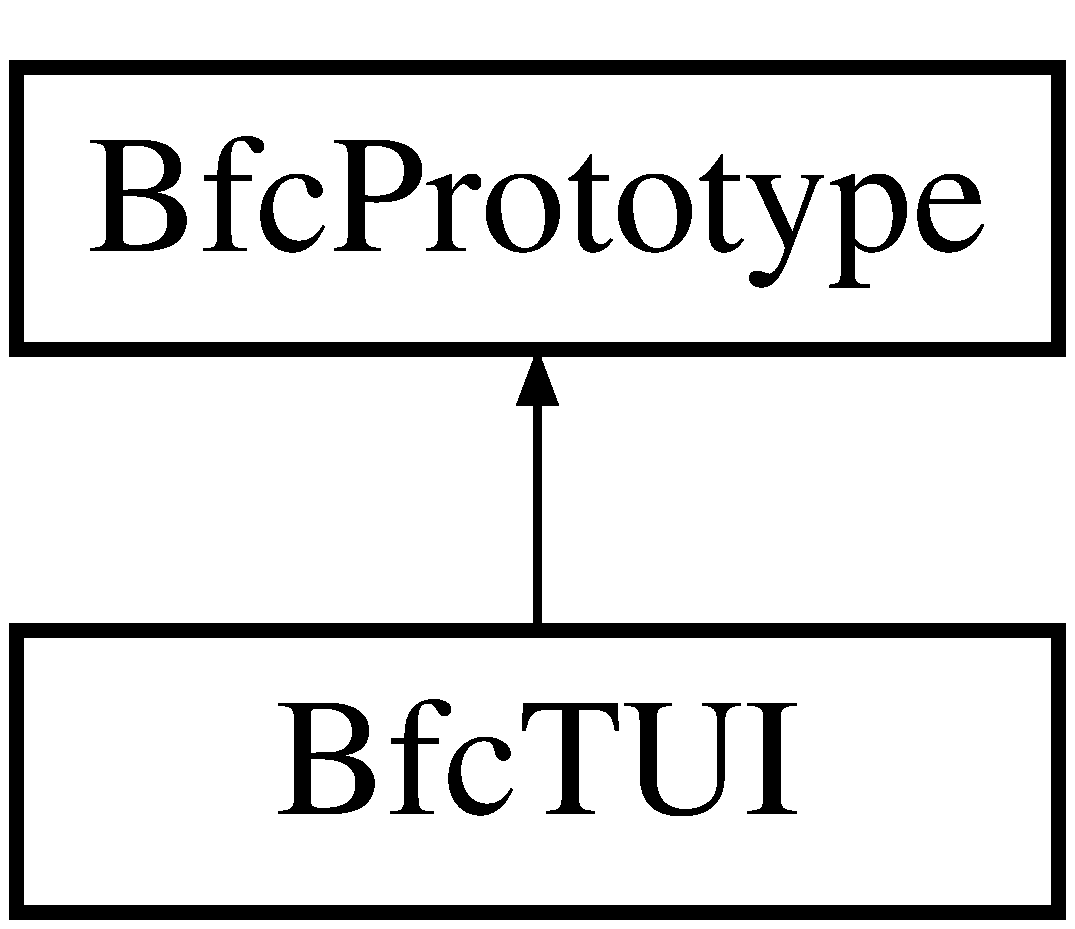
\includegraphics[height=2.000000cm]{classBfcTUI}
\end{center}
\end{figure}
\subsection*{Public Member Functions}
\begin{DoxyCompactItemize}
\item 
\hyperlink{classBfcTUI_aec4a74685e13990672018efe38f63cd8}{Bfc\-T\-U\-I} ()
\item 
\hyperlink{classBfcTUI_adff8e447a86fd73ead506f7d4da38646}{$\sim$\-Bfc\-T\-U\-I} ()
\item 
void \hyperlink{classBfcTUI_a4034a1a0e50d24ca3da16683ca7a0bd1}{print\-Day} (std\-::ostream \&os, \hyperlink{classDate}{Date} d, int width)
\item 
void \hyperlink{classBfcTUI_a50402f167049c054ba2512374e7e0b03}{show\-Record} (std\-::ostream \&os, std\-::vector$<$ \hyperlink{classTask}{Task} $>$ \&ts, int s)
\item 
void \hyperlink{classBfcTUI_a1c446b91f4f250d4b4f5f255e207c88e}{write\-Record} (std\-::ostream \&os, std\-::vector$<$ \hyperlink{classTask}{Task} $>$ \&ts)
\item 
void \hyperlink{classBfcTUI_a5577e09a7a8b9df3d4ab1edf8bcdd5f4}{brief\-Report} (std\-::ostream \&os, std\-::vector$<$ \hyperlink{classTask}{Task} $>$ \&ts)
\item 
void \hyperlink{classBfcTUI_a816b7be298cd8f33001748f1d54b4297}{timeline} (std\-::ostream \&os, std\-::vector$<$ \hyperlink{classTask}{Task} $>$ \&ts, \hyperlink{classDate}{Date} s, \hyperlink{classDate}{Date} e, bool m)
\end{DoxyCompactItemize}
\subsection*{Private Member Functions}
\begin{DoxyCompactItemize}
\item 
void \hyperlink{classBfcTUI_a3803d34ecb5b2e8389a04bd07cc55d3c}{timeline\-Ver} (std\-::ostream \&os, std\-::vector$<$ \hyperlink{classTask}{Task} $>$ \&ts, \hyperlink{classDate}{Date} s, \hyperlink{classDate}{Date} e)
\item 
void \hyperlink{classBfcTUI_aeddc5da12ada09fa9e4bbb7f135bdda9}{timeline\-Hor} (std\-::ostream \&os, std\-::vector$<$ \hyperlink{classTask}{Task} $>$ \&ts, \hyperlink{classDate}{Date} s, \hyperlink{classDate}{Date} e)
\end{DoxyCompactItemize}
\subsection*{Additional Inherited Members}


\subsection{Detailed Description}
\hyperlink{classBfcTUI}{Bfc\-T\-U\-I} Class is inherited from \hyperlink{classBfcPrototype}{Bfc\-Prototype}. 

\hyperlink{classBfcTUI}{Bfc\-T\-U\-I} provides some interesting functions to build the text-\/based U\-I This is one main variant of the Bacpfsec Project main 

\subsection{Constructor \& Destructor Documentation}
\hypertarget{classBfcTUI_aec4a74685e13990672018efe38f63cd8}{\index{Bfc\-T\-U\-I@{Bfc\-T\-U\-I}!Bfc\-T\-U\-I@{Bfc\-T\-U\-I}}
\index{Bfc\-T\-U\-I@{Bfc\-T\-U\-I}!BfcTUI@{Bfc\-T\-U\-I}}
\subsubsection[{Bfc\-T\-U\-I}]{\setlength{\rightskip}{0pt plus 5cm}Bfc\-T\-U\-I\-::\-Bfc\-T\-U\-I (
\begin{DoxyParamCaption}
{}
\end{DoxyParamCaption}
)}}\label{classBfcTUI_aec4a74685e13990672018efe38f63cd8}
Default constructor \hypertarget{classBfcTUI_adff8e447a86fd73ead506f7d4da38646}{\index{Bfc\-T\-U\-I@{Bfc\-T\-U\-I}!$\sim$\-Bfc\-T\-U\-I@{$\sim$\-Bfc\-T\-U\-I}}
\index{$\sim$\-Bfc\-T\-U\-I@{$\sim$\-Bfc\-T\-U\-I}!BfcTUI@{Bfc\-T\-U\-I}}
\subsubsection[{$\sim$\-Bfc\-T\-U\-I}]{\setlength{\rightskip}{0pt plus 5cm}Bfc\-T\-U\-I\-::$\sim$\-Bfc\-T\-U\-I (
\begin{DoxyParamCaption}
{}
\end{DoxyParamCaption}
)}}\label{classBfcTUI_adff8e447a86fd73ead506f7d4da38646}
Destructor 

\subsection{Member Function Documentation}
\hypertarget{classBfcTUI_a5577e09a7a8b9df3d4ab1edf8bcdd5f4}{\index{Bfc\-T\-U\-I@{Bfc\-T\-U\-I}!brief\-Report@{brief\-Report}}
\index{brief\-Report@{brief\-Report}!BfcTUI@{Bfc\-T\-U\-I}}
\subsubsection[{brief\-Report}]{\setlength{\rightskip}{0pt plus 5cm}void Bfc\-T\-U\-I\-::brief\-Report (
\begin{DoxyParamCaption}
\item[{std\-::ostream \&}]{os, }
\item[{std\-::vector$<$ {\bf Task} $>$ \&}]{ts}
\end{DoxyParamCaption}
)}}\label{classBfcTUI_a5577e09a7a8b9df3d4ab1edf8bcdd5f4}
brief\-Report to ostream 
\begin{DoxyParams}{Parameters}
{\em os} & ostream \\
\hline
{\em ts} & reference to a task vector \\
\hline
\end{DoxyParams}
\hypertarget{classBfcTUI_a4034a1a0e50d24ca3da16683ca7a0bd1}{\index{Bfc\-T\-U\-I@{Bfc\-T\-U\-I}!print\-Day@{print\-Day}}
\index{print\-Day@{print\-Day}!BfcTUI@{Bfc\-T\-U\-I}}
\subsubsection[{print\-Day}]{\setlength{\rightskip}{0pt plus 5cm}void Bfc\-T\-U\-I\-::print\-Day (
\begin{DoxyParamCaption}
\item[{std\-::ostream \&}]{os, }
\item[{{\bf Date}}]{d, }
\item[{int}]{width}
\end{DoxyParamCaption}
)}}\label{classBfcTUI_a4034a1a0e50d24ca3da16683ca7a0bd1}
Print given date with given width 
\begin{DoxyParams}{Parameters}
{\em os} & ostream \\
\hline
{\em d} & a \hyperlink{classDate}{Date} object \\
\hline
{\em witth} & desired output width \\
\hline
\end{DoxyParams}
\hypertarget{classBfcTUI_a50402f167049c054ba2512374e7e0b03}{\index{Bfc\-T\-U\-I@{Bfc\-T\-U\-I}!show\-Record@{show\-Record}}
\index{show\-Record@{show\-Record}!BfcTUI@{Bfc\-T\-U\-I}}
\subsubsection[{show\-Record}]{\setlength{\rightskip}{0pt plus 5cm}void Bfc\-T\-U\-I\-::show\-Record (
\begin{DoxyParamCaption}
\item[{std\-::ostream \&}]{os, }
\item[{std\-::vector$<$ {\bf Task} $>$ \&}]{ts, }
\item[{int}]{s}
\end{DoxyParamCaption}
)}}\label{classBfcTUI_a50402f167049c054ba2512374e7e0b03}
show\-Record to ostream 
\begin{DoxyParams}{Parameters}
{\em os} & ostream \\
\hline
{\em ts} & reference to a task vector \\
\hline
{\em s} & status integer \\
\hline
\end{DoxyParams}
\hypertarget{classBfcTUI_a816b7be298cd8f33001748f1d54b4297}{\index{Bfc\-T\-U\-I@{Bfc\-T\-U\-I}!timeline@{timeline}}
\index{timeline@{timeline}!BfcTUI@{Bfc\-T\-U\-I}}
\subsubsection[{timeline}]{\setlength{\rightskip}{0pt plus 5cm}void Bfc\-T\-U\-I\-::timeline (
\begin{DoxyParamCaption}
\item[{std\-::ostream \&}]{os, }
\item[{std\-::vector$<$ {\bf Task} $>$ \&}]{ts, }
\item[{{\bf Date}}]{s, }
\item[{{\bf Date}}]{e, }
\item[{bool}]{m}
\end{DoxyParamCaption}
)}}\label{classBfcTUI_a816b7be298cd8f33001748f1d54b4297}
timeline function with variant 
\begin{DoxyParams}{Parameters}
{\em os} & ostream \\
\hline
{\em ts} & reference to a task vector \\
\hline
{\em s} & start \hyperlink{classDate}{Date} input from user \\
\hline
{\em e} & end \hyperlink{classDate}{Date} input from user \\
\hline
{\em m} & boolean selector, 0\-:horizontal, 1\-:vertical \\
\hline
\end{DoxyParams}
\hypertarget{classBfcTUI_aeddc5da12ada09fa9e4bbb7f135bdda9}{\index{Bfc\-T\-U\-I@{Bfc\-T\-U\-I}!timeline\-Hor@{timeline\-Hor}}
\index{timeline\-Hor@{timeline\-Hor}!BfcTUI@{Bfc\-T\-U\-I}}
\subsubsection[{timeline\-Hor}]{\setlength{\rightskip}{0pt plus 5cm}void Bfc\-T\-U\-I\-::timeline\-Hor (
\begin{DoxyParamCaption}
\item[{std\-::ostream \&}]{os, }
\item[{std\-::vector$<$ {\bf Task} $>$ \&}]{ts, }
\item[{{\bf Date}}]{s, }
\item[{{\bf Date}}]{e}
\end{DoxyParamCaption}
)\hspace{0.3cm}{\ttfamily [private]}}}\label{classBfcTUI_aeddc5da12ada09fa9e4bbb7f135bdda9}
Private helper to build horizontal timeline 
\begin{DoxyParams}{Parameters}
{\em os} & ostream \\
\hline
{\em ts} & reference to a task vector \\
\hline
{\em s} & start \hyperlink{classDate}{Date} input from user \\
\hline
{\em e} & end \hyperlink{classDate}{Date} input from user \\
\hline
\end{DoxyParams}
\hypertarget{classBfcTUI_a3803d34ecb5b2e8389a04bd07cc55d3c}{\index{Bfc\-T\-U\-I@{Bfc\-T\-U\-I}!timeline\-Ver@{timeline\-Ver}}
\index{timeline\-Ver@{timeline\-Ver}!BfcTUI@{Bfc\-T\-U\-I}}
\subsubsection[{timeline\-Ver}]{\setlength{\rightskip}{0pt plus 5cm}void Bfc\-T\-U\-I\-::timeline\-Ver (
\begin{DoxyParamCaption}
\item[{std\-::ostream \&}]{os, }
\item[{std\-::vector$<$ {\bf Task} $>$ \&}]{ts, }
\item[{{\bf Date}}]{s, }
\item[{{\bf Date}}]{e}
\end{DoxyParamCaption}
)\hspace{0.3cm}{\ttfamily [private]}}}\label{classBfcTUI_a3803d34ecb5b2e8389a04bd07cc55d3c}
Private helper to build vertical timeline 
\begin{DoxyParams}{Parameters}
{\em os} & ostream \\
\hline
{\em ts} & reference to a task vector \\
\hline
{\em s} & start \hyperlink{classDate}{Date} input from user \\
\hline
{\em e} & end \hyperlink{classDate}{Date} input from user \\
\hline
\end{DoxyParams}
\hypertarget{classBfcTUI_a1c446b91f4f250d4b4f5f255e207c88e}{\index{Bfc\-T\-U\-I@{Bfc\-T\-U\-I}!write\-Record@{write\-Record}}
\index{write\-Record@{write\-Record}!BfcTUI@{Bfc\-T\-U\-I}}
\subsubsection[{write\-Record}]{\setlength{\rightskip}{0pt plus 5cm}void Bfc\-T\-U\-I\-::write\-Record (
\begin{DoxyParamCaption}
\item[{std\-::ostream \&}]{os, }
\item[{std\-::vector$<$ {\bf Task} $>$ \&}]{ts}
\end{DoxyParamCaption}
)}}\label{classBfcTUI_a1c446b91f4f250d4b4f5f255e207c88e}
write\-Record to ostream 
\begin{DoxyParams}{Parameters}
{\em os} & ostream \\
\hline
{\em ts} & reference to a task vector \\
\hline
\end{DoxyParams}


The documentation for this class was generated from the following files\-:\begin{DoxyCompactItemize}
\item 
\hyperlink{BfcTUI_8h}{Bfc\-T\-U\-I.\-h}\item 
\hyperlink{BfcTUI_8cc}{Bfc\-T\-U\-I.\-cc}\end{DoxyCompactItemize}

\hypertarget{classDate}{\section{Date Class Reference}
\label{classDate}\index{Date@{Date}}
}


\hyperlink{classDate}{Date} Class is used for time recording.  




{\ttfamily \#include $<$Date.\-h$>$}

\subsection*{Public Member Functions}
\begin{DoxyCompactItemize}
\item 
\hyperlink{classDate_a4e59ed4ba66eec61c27460c5d09fa1bd}{Date} ()
\item 
\hyperlink{classDate_a86d5d0d04d211f5fa077386de1ce7f19}{Date} (int d)
\item 
\hyperlink{classDate_a2233b93eaed1626e957435cedfc511de}{Date} (const \hyperlink{classDate}{Date} \&dt)
\item 
\hyperlink{classDate_ade4b469433b7966cc034cbcc6799233b}{$\sim$\-Date} ()
\item 
void \hyperlink{classDate_a33ea2c0c7bd11cc5fa95ad7d346fcff4}{set\-Value} (int d)
\item 
int \hyperlink{classDate_ab92e73e4246833b2e66b373ef3fefdf0}{get\-Value} ()
\item 
void \hyperlink{classDate_a689d13b5e5882068308b02073e1ed321}{next\-Date} ()
\item 
bool \hyperlink{classDate_a0036e87463cdee6117d27f04933393fb}{operator==} (\hyperlink{classDate}{Date} d)
\item 
bool \hyperlink{classDate_a5d7fa843430ed6a618b104b2f9ce8f03}{operator!=} (\hyperlink{classDate}{Date} d)
\end{DoxyCompactItemize}
\subsection*{Private Member Functions}
\begin{DoxyCompactItemize}
\item 
bool \hyperlink{classDate_a7d9aaa9db591413e21c8b85fdae130ad}{is\-Valid} ()
\end{DoxyCompactItemize}
\subsection*{Private Attributes}
\begin{DoxyCompactItemize}
\item 
int \hyperlink{classDate_abfe1e095c0de4e7d1ce6ae1ac97026d5}{date}
\end{DoxyCompactItemize}


\subsection{Detailed Description}
\hyperlink{classDate}{Date} Class is used for time recording. 

\hyperlink{classDate}{Date} Class provides supplementary operations based on the $<$time$>$ library 

\subsection{Constructor \& Destructor Documentation}
\hypertarget{classDate_a4e59ed4ba66eec61c27460c5d09fa1bd}{\index{Date@{Date}!Date@{Date}}
\index{Date@{Date}!Date@{Date}}
\subsubsection[{Date}]{\setlength{\rightskip}{0pt plus 5cm}Date\-::\-Date (
\begin{DoxyParamCaption}
{}
\end{DoxyParamCaption}
)}}\label{classDate_a4e59ed4ba66eec61c27460c5d09fa1bd}
Default constructor \begin{DoxyNote}{Note}
Default value is 150301 (i.\-e. 2015/03/01) 
\end{DoxyNote}
\hypertarget{classDate_a86d5d0d04d211f5fa077386de1ce7f19}{\index{Date@{Date}!Date@{Date}}
\index{Date@{Date}!Date@{Date}}
\subsubsection[{Date}]{\setlength{\rightskip}{0pt plus 5cm}Date\-::\-Date (
\begin{DoxyParamCaption}
\item[{int}]{d}
\end{DoxyParamCaption}
)}}\label{classDate_a86d5d0d04d211f5fa077386de1ce7f19}
Parameterized constructor 
\begin{DoxyParams}{Parameters}
{\em d} & Value stands for a date \\
\hline
\end{DoxyParams}
set back to default for invalid date \hypertarget{classDate_a2233b93eaed1626e957435cedfc511de}{\index{Date@{Date}!Date@{Date}}
\index{Date@{Date}!Date@{Date}}
\subsubsection[{Date}]{\setlength{\rightskip}{0pt plus 5cm}Date\-::\-Date (
\begin{DoxyParamCaption}
\item[{const {\bf Date} \&}]{dt}
\end{DoxyParamCaption}
)}}\label{classDate_a2233b93eaed1626e957435cedfc511de}
Copy constructor \hypertarget{classDate_ade4b469433b7966cc034cbcc6799233b}{\index{Date@{Date}!$\sim$\-Date@{$\sim$\-Date}}
\index{$\sim$\-Date@{$\sim$\-Date}!Date@{Date}}
\subsubsection[{$\sim$\-Date}]{\setlength{\rightskip}{0pt plus 5cm}Date\-::$\sim$\-Date (
\begin{DoxyParamCaption}
{}
\end{DoxyParamCaption}
)}}\label{classDate_ade4b469433b7966cc034cbcc6799233b}
Destructor 

\subsection{Member Function Documentation}
\hypertarget{classDate_ab92e73e4246833b2e66b373ef3fefdf0}{\index{Date@{Date}!get\-Value@{get\-Value}}
\index{get\-Value@{get\-Value}!Date@{Date}}
\subsubsection[{get\-Value}]{\setlength{\rightskip}{0pt plus 5cm}int Date\-::get\-Value (
\begin{DoxyParamCaption}
{}
\end{DoxyParamCaption}
)}}\label{classDate_ab92e73e4246833b2e66b373ef3fefdf0}
Getter \begin{DoxyReturn}{Returns}
Value of the private date 
\end{DoxyReturn}
\hypertarget{classDate_a7d9aaa9db591413e21c8b85fdae130ad}{\index{Date@{Date}!is\-Valid@{is\-Valid}}
\index{is\-Valid@{is\-Valid}!Date@{Date}}
\subsubsection[{is\-Valid}]{\setlength{\rightskip}{0pt plus 5cm}bool Date\-::is\-Valid (
\begin{DoxyParamCaption}
{}
\end{DoxyParamCaption}
)\hspace{0.3cm}{\ttfamily [private]}}}\label{classDate_a7d9aaa9db591413e21c8b85fdae130ad}
\hyperlink{classDate}{Date} check

Private helper to test if a date is valid \hypertarget{classDate_a689d13b5e5882068308b02073e1ed321}{\index{Date@{Date}!next\-Date@{next\-Date}}
\index{next\-Date@{next\-Date}!Date@{Date}}
\subsubsection[{next\-Date}]{\setlength{\rightskip}{0pt plus 5cm}void Date\-::next\-Date (
\begin{DoxyParamCaption}
{}
\end{DoxyParamCaption}
)}}\label{classDate_a689d13b5e5882068308b02073e1ed321}
Proceed date to next valid date \hypertarget{classDate_a5d7fa843430ed6a618b104b2f9ce8f03}{\index{Date@{Date}!operator!=@{operator!=}}
\index{operator!=@{operator!=}!Date@{Date}}
\subsubsection[{operator!=}]{\setlength{\rightskip}{0pt plus 5cm}bool Date\-::operator!= (
\begin{DoxyParamCaption}
\item[{{\bf Date}}]{d}
\end{DoxyParamCaption}
)}}\label{classDate_a5d7fa843430ed6a618b104b2f9ce8f03}
Overload != operator param d another date \hypertarget{classDate_a0036e87463cdee6117d27f04933393fb}{\index{Date@{Date}!operator==@{operator==}}
\index{operator==@{operator==}!Date@{Date}}
\subsubsection[{operator==}]{\setlength{\rightskip}{0pt plus 5cm}bool Date\-::operator== (
\begin{DoxyParamCaption}
\item[{{\bf Date}}]{d}
\end{DoxyParamCaption}
)}}\label{classDate_a0036e87463cdee6117d27f04933393fb}
Overload == operator param d another date \hypertarget{classDate_a33ea2c0c7bd11cc5fa95ad7d346fcff4}{\index{Date@{Date}!set\-Value@{set\-Value}}
\index{set\-Value@{set\-Value}!Date@{Date}}
\subsubsection[{set\-Value}]{\setlength{\rightskip}{0pt plus 5cm}void Date\-::set\-Value (
\begin{DoxyParamCaption}
\item[{int}]{d}
\end{DoxyParamCaption}
)}}\label{classDate_a33ea2c0c7bd11cc5fa95ad7d346fcff4}
Setter 
\begin{DoxyParams}{Parameters}
{\em d} & Value stands for a date \\
\hline
\end{DoxyParams}


\subsection{Member Data Documentation}
\hypertarget{classDate_abfe1e095c0de4e7d1ce6ae1ac97026d5}{\index{Date@{Date}!date@{date}}
\index{date@{date}!Date@{Date}}
\subsubsection[{date}]{\setlength{\rightskip}{0pt plus 5cm}int Date\-::date\hspace{0.3cm}{\ttfamily [private]}}}\label{classDate_abfe1e095c0de4e7d1ce6ae1ac97026d5}
Storage of date value 

The documentation for this class was generated from the following files\-:\begin{DoxyCompactItemize}
\item 
\hyperlink{Date_8h}{Date.\-h}\item 
\hyperlink{Date_8cc}{Date.\-cc}\end{DoxyCompactItemize}

\hypertarget{classFixtureBfcPrototype}{\section{Fixture\-Bfc\-Prototype Class Reference}
\label{classFixtureBfcPrototype}\index{Fixture\-Bfc\-Prototype@{Fixture\-Bfc\-Prototype}}
}
Inheritance diagram for Fixture\-Bfc\-Prototype\-:\begin{figure}[H]
\begin{center}
\leavevmode
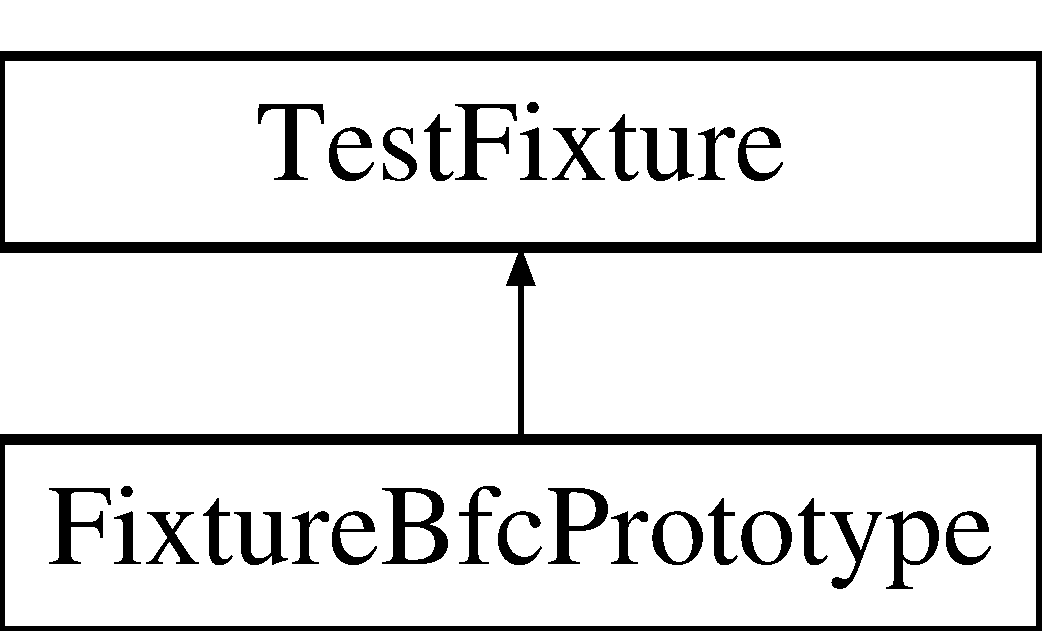
\includegraphics[height=2.000000cm]{classFixtureBfcPrototype}
\end{center}
\end{figure}
\subsection*{Public Member Functions}
\begin{DoxyCompactItemize}
\item 
\hypertarget{classFixtureBfcPrototype_a9c1674fb8052ab26caebd4fae98af62a}{{\bfseries C\-P\-P\-U\-N\-I\-T\-\_\-\-T\-E\-S\-T\-\_\-\-S\-U\-I\-T\-E} (\hyperlink{classFixtureBfcPrototype}{Fixture\-Bfc\-Prototype})}\label{classFixtureBfcPrototype_a9c1674fb8052ab26caebd4fae98af62a}

\item 
\hypertarget{classFixtureBfcPrototype_a1dd89fce7cad542802ab43719ab61428}{{\bfseries C\-P\-P\-U\-N\-I\-T\-\_\-\-T\-E\-S\-T} (\hyperlink{classFixtureBfcPrototype_ae31927f6a2e426d63c84df84986b524f}{test\-Init\-And\-Getters})}\label{classFixtureBfcPrototype_a1dd89fce7cad542802ab43719ab61428}

\item 
\hypertarget{classFixtureBfcPrototype_a584af8672bf83affd1d54ba96fe07318}{{\bfseries C\-P\-P\-U\-N\-I\-T\-\_\-\-T\-E\-S\-T} (\hyperlink{classFixtureBfcPrototype_a0b23c11f05550525697ef00225c35d26}{test\-Setters})}\label{classFixtureBfcPrototype_a584af8672bf83affd1d54ba96fe07318}

\item 
\hypertarget{classFixtureBfcPrototype_ad899807a5e9aa77930190db2c6b247ed}{{\bfseries C\-P\-P\-U\-N\-I\-T\-\_\-\-T\-E\-S\-T} (\hyperlink{classFixtureBfcPrototype_addf464a098f84fa974297bbfd5c6ff61}{test\-Tasks\-Getter})}\label{classFixtureBfcPrototype_ad899807a5e9aa77930190db2c6b247ed}

\item 
\hypertarget{classFixtureBfcPrototype_a0582ec432738e71042a44b04f4e6ab78}{{\bfseries C\-P\-P\-U\-N\-I\-T\-\_\-\-T\-E\-S\-T} (\hyperlink{classFixtureBfcPrototype_ab2a742a030f3aff0e15721558bca6792}{test\-Read\-States})}\label{classFixtureBfcPrototype_a0582ec432738e71042a44b04f4e6ab78}

\item 
\hypertarget{classFixtureBfcPrototype_a120e0333893dba1dd349bf2914d78255}{{\bfseries C\-P\-P\-U\-N\-I\-T\-\_\-\-T\-E\-S\-T} (\hyperlink{classFixtureBfcPrototype_a5f91dcaef614e6c5b6af4a374de69bf9}{test\-Read\-Tasks})}\label{classFixtureBfcPrototype_a120e0333893dba1dd349bf2914d78255}

\item 
\hypertarget{classFixtureBfcPrototype_a4ace544e960a56b8e4b568b36110c857}{{\bfseries C\-P\-P\-U\-N\-I\-T\-\_\-\-T\-E\-S\-T\-\_\-\-S\-U\-I\-T\-E\-\_\-\-E\-N\-D} ()}\label{classFixtureBfcPrototype_a4ace544e960a56b8e4b568b36110c857}

\item 
\hypertarget{classFixtureBfcPrototype_a4ed11dbe79642d1c4d25341e19d625ee}{void {\bfseries set\-Up} ()}\label{classFixtureBfcPrototype_a4ed11dbe79642d1c4d25341e19d625ee}

\item 
\hypertarget{classFixtureBfcPrototype_a752d86ee40b060929a754540a0ee96dc}{void {\bfseries tear\-Down} ()}\label{classFixtureBfcPrototype_a752d86ee40b060929a754540a0ee96dc}

\item 
void \hyperlink{classFixtureBfcPrototype_ae31927f6a2e426d63c84df84986b524f}{test\-Init\-And\-Getters} ()
\item 
void \hyperlink{classFixtureBfcPrototype_a0b23c11f05550525697ef00225c35d26}{test\-Setters} ()
\item 
void \hyperlink{classFixtureBfcPrototype_addf464a098f84fa974297bbfd5c6ff61}{test\-Tasks\-Getter} ()
\item 
void \hyperlink{classFixtureBfcPrototype_ab2a742a030f3aff0e15721558bca6792}{test\-Read\-States} ()
\item 
void \hyperlink{classFixtureBfcPrototype_a5f91dcaef614e6c5b6af4a374de69bf9}{test\-Read\-Tasks} ()
\end{DoxyCompactItemize}
\subsection*{Private Attributes}
\begin{DoxyCompactItemize}
\item 
\hypertarget{classFixtureBfcPrototype_a90321d4640e0c5c6ce383368ff1e70e7}{\hyperlink{classBfcPrototype}{Bfc\-Prototype} $\ast$ {\bfseries bfc}}\label{classFixtureBfcPrototype_a90321d4640e0c5c6ce383368ff1e70e7}

\end{DoxyCompactItemize}


\subsection{Member Function Documentation}
\hypertarget{classFixtureBfcPrototype_ae31927f6a2e426d63c84df84986b524f}{\index{Fixture\-Bfc\-Prototype@{Fixture\-Bfc\-Prototype}!test\-Init\-And\-Getters@{test\-Init\-And\-Getters}}
\index{test\-Init\-And\-Getters@{test\-Init\-And\-Getters}!FixtureBfcPrototype@{Fixture\-Bfc\-Prototype}}
\subsubsection[{test\-Init\-And\-Getters}]{\setlength{\rightskip}{0pt plus 5cm}void Fixture\-Bfc\-Prototype\-::test\-Init\-And\-Getters (
\begin{DoxyParamCaption}
{}
\end{DoxyParamCaption}
)\hspace{0.3cm}{\ttfamily [inline]}}}\label{classFixtureBfcPrototype_ae31927f6a2e426d63c84df84986b524f}
Tests for Getters and init

Test1\-: get\-Record\-Loaded() Test2\-: get\-Start\-Date() Test3\-: get\-End\-Date() Test4\-: get\-Num\-Of\-Task\-Uncomplete() Test5\-: get\-Num\-Of\-Task\-Cancelled() \hypertarget{classFixtureBfcPrototype_ab2a742a030f3aff0e15721558bca6792}{\index{Fixture\-Bfc\-Prototype@{Fixture\-Bfc\-Prototype}!test\-Read\-States@{test\-Read\-States}}
\index{test\-Read\-States@{test\-Read\-States}!FixtureBfcPrototype@{Fixture\-Bfc\-Prototype}}
\subsubsection[{test\-Read\-States}]{\setlength{\rightskip}{0pt plus 5cm}void Fixture\-Bfc\-Prototype\-::test\-Read\-States (
\begin{DoxyParamCaption}
{}
\end{DoxyParamCaption}
)\hspace{0.3cm}{\ttfamily [inline]}}}\label{classFixtureBfcPrototype_ab2a742a030f3aff0e15721558bca6792}
Test for Bfc\-Prototype\-::read\-States(istream, Task\&)

Test input\-: \mbox{[} $\sim$\-P2 \mbox{]} 20150302 \mbox{[} $\sim$\-P3 + $\sim$\-P5 \mbox{]} 20150304 1 \hypertarget{classFixtureBfcPrototype_a5f91dcaef614e6c5b6af4a374de69bf9}{\index{Fixture\-Bfc\-Prototype@{Fixture\-Bfc\-Prototype}!test\-Read\-Tasks@{test\-Read\-Tasks}}
\index{test\-Read\-Tasks@{test\-Read\-Tasks}!FixtureBfcPrototype@{Fixture\-Bfc\-Prototype}}
\subsubsection[{test\-Read\-Tasks}]{\setlength{\rightskip}{0pt plus 5cm}void Fixture\-Bfc\-Prototype\-::test\-Read\-Tasks (
\begin{DoxyParamCaption}
{}
\end{DoxyParamCaption}
)\hspace{0.3cm}{\ttfamily [inline]}}}\label{classFixtureBfcPrototype_a5f91dcaef614e6c5b6af4a374de69bf9}
Test for Bfc\-Prototype\-::read\-States(istream, vector$<$\-Task$>$\&)

Test input\-: Book1 \mbox{[} $\sim$\-P2 \mbox{]} 20150302 \mbox{[} $\sim$\-P3 + $\sim$\-P5 \mbox{]} 20150304 1 Book2 \mbox{[} $\sim$\-C1 \mbox{]} 20150101 \mbox{[} $\sim$\-C3 \mbox{]} 20150502 0 \hypertarget{classFixtureBfcPrototype_a0b23c11f05550525697ef00225c35d26}{\index{Fixture\-Bfc\-Prototype@{Fixture\-Bfc\-Prototype}!test\-Setters@{test\-Setters}}
\index{test\-Setters@{test\-Setters}!FixtureBfcPrototype@{Fixture\-Bfc\-Prototype}}
\subsubsection[{test\-Setters}]{\setlength{\rightskip}{0pt plus 5cm}void Fixture\-Bfc\-Prototype\-::test\-Setters (
\begin{DoxyParamCaption}
{}
\end{DoxyParamCaption}
)\hspace{0.3cm}{\ttfamily [inline]}}}\label{classFixtureBfcPrototype_a0b23c11f05550525697ef00225c35d26}
Tests for Setters

Test1\-: set\-Record\-Loaded() Test2\-: set\-Start\-Date() Test3\-: set\-End\-Date() Test4\-: set\-Num\-Of\-Task\-Uncomplete() Test5\-: set\-Num\-Of\-Task\-Cancelled() \hypertarget{classFixtureBfcPrototype_addf464a098f84fa974297bbfd5c6ff61}{\index{Fixture\-Bfc\-Prototype@{Fixture\-Bfc\-Prototype}!test\-Tasks\-Getter@{test\-Tasks\-Getter}}
\index{test\-Tasks\-Getter@{test\-Tasks\-Getter}!FixtureBfcPrototype@{Fixture\-Bfc\-Prototype}}
\subsubsection[{test\-Tasks\-Getter}]{\setlength{\rightskip}{0pt plus 5cm}void Fixture\-Bfc\-Prototype\-::test\-Tasks\-Getter (
\begin{DoxyParamCaption}
{}
\end{DoxyParamCaption}
)\hspace{0.3cm}{\ttfamily [inline]}}}\label{classFixtureBfcPrototype_addf464a098f84fa974297bbfd5c6ff61}
Test for \hyperlink{classBfcPrototype_a414637b5643f0ef2a8834d1d591da364}{Bfc\-Prototype\-::get\-Tasks()} 

The documentation for this class was generated from the following file\-:\begin{DoxyCompactItemize}
\item 
\hyperlink{FixtureBfcPrototype_8h}{Fixture\-Bfc\-Prototype.\-h}\end{DoxyCompactItemize}

\hypertarget{classFixtureBfcTUI}{\section{Fixture\-Bfc\-T\-U\-I Class Reference}
\label{classFixtureBfcTUI}\index{Fixture\-Bfc\-T\-U\-I@{Fixture\-Bfc\-T\-U\-I}}
}
Inheritance diagram for Fixture\-Bfc\-T\-U\-I\-:\begin{figure}[H]
\begin{center}
\leavevmode
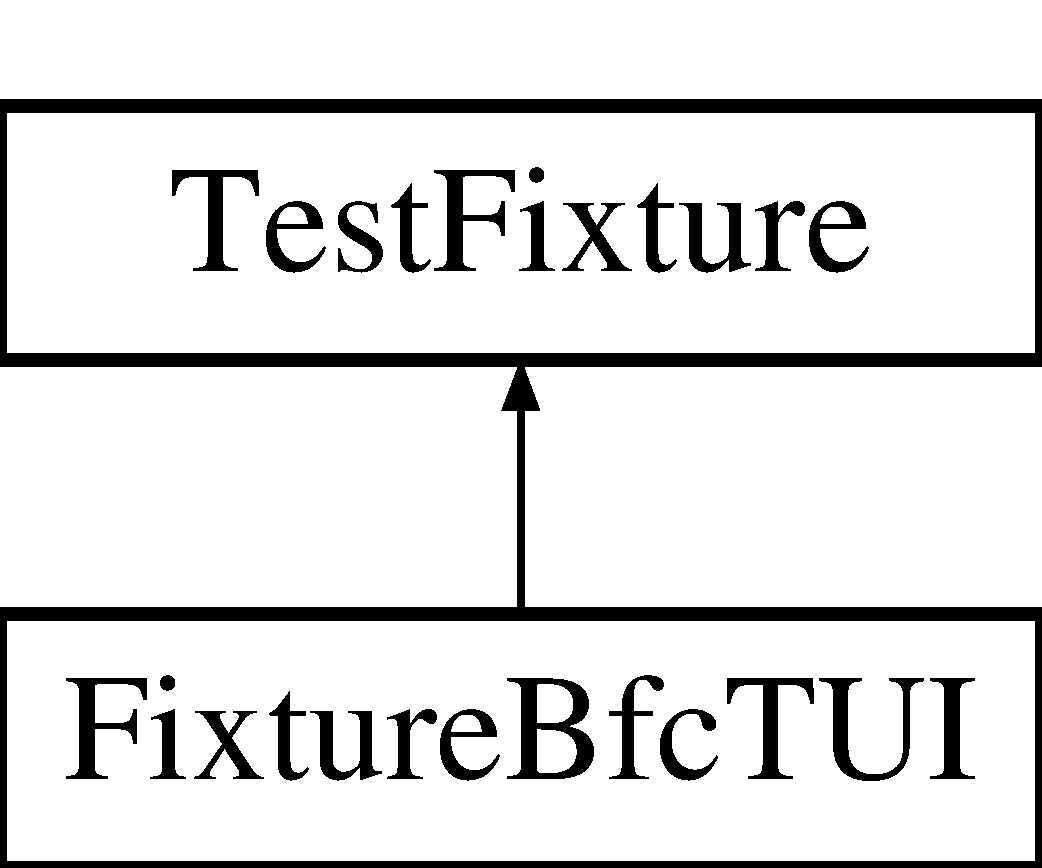
\includegraphics[height=2.000000cm]{classFixtureBfcTUI}
\end{center}
\end{figure}
\subsection*{Public Member Functions}
\begin{DoxyCompactItemize}
\item 
\hypertarget{classFixtureBfcTUI_a203ae36ccef8d8180139343760c0dbdc}{{\bfseries C\-P\-P\-U\-N\-I\-T\-\_\-\-T\-E\-S\-T\-\_\-\-S\-U\-I\-T\-E} (\hyperlink{classFixtureBfcTUI}{Fixture\-Bfc\-T\-U\-I})}\label{classFixtureBfcTUI_a203ae36ccef8d8180139343760c0dbdc}

\item 
\hypertarget{classFixtureBfcTUI_ac5002cbc63f5e0eb860d5cda9c2f5789}{{\bfseries C\-P\-P\-U\-N\-I\-T\-\_\-\-T\-E\-S\-T} (\hyperlink{classFixtureBfcTUI_a0e6e249a57e8679db2fe58e606986b95}{test\-Print\-Day})}\label{classFixtureBfcTUI_ac5002cbc63f5e0eb860d5cda9c2f5789}

\item 
\hypertarget{classFixtureBfcTUI_ad5af97d2673839a8b547b29d37140885}{{\bfseries C\-P\-P\-U\-N\-I\-T\-\_\-\-T\-E\-S\-T} (\hyperlink{classFixtureBfcTUI_a8b307755f136be0db22d450e9724bf2a}{test\-Show\-Record})}\label{classFixtureBfcTUI_ad5af97d2673839a8b547b29d37140885}

\item 
\hypertarget{classFixtureBfcTUI_a5849bb2ffaf03cef983c266479e567da}{{\bfseries C\-P\-P\-U\-N\-I\-T\-\_\-\-T\-E\-S\-T} (\hyperlink{classFixtureBfcTUI_a4a099462414f1ee59f0458e7ba35857f}{test\-Write\-Record})}\label{classFixtureBfcTUI_a5849bb2ffaf03cef983c266479e567da}

\item 
\hypertarget{classFixtureBfcTUI_abc4ba04e15fcdc7af67050538bc4384c}{{\bfseries C\-P\-P\-U\-N\-I\-T\-\_\-\-T\-E\-S\-T} (\hyperlink{classFixtureBfcTUI_adbbb524adf16d7057835ea25c4a13369}{test\-Brief\-Report})}\label{classFixtureBfcTUI_abc4ba04e15fcdc7af67050538bc4384c}

\item 
\hypertarget{classFixtureBfcTUI_a6cc3b1f974d90f81352ecd3b92633d17}{{\bfseries C\-P\-P\-U\-N\-I\-T\-\_\-\-T\-E\-S\-T} (\hyperlink{classFixtureBfcTUI_aef00e5a6e84b832da4ec58aa1f804d33}{test\-Timeline\-Ver})}\label{classFixtureBfcTUI_a6cc3b1f974d90f81352ecd3b92633d17}

\item 
\hypertarget{classFixtureBfcTUI_a6329e91e6764611b1172fd243f2404ec}{{\bfseries C\-P\-P\-U\-N\-I\-T\-\_\-\-T\-E\-S\-T} (\hyperlink{classFixtureBfcTUI_a84e72246b10ab731470fcb9818f452e2}{test\-Timeline\-Hor})}\label{classFixtureBfcTUI_a6329e91e6764611b1172fd243f2404ec}

\item 
\hypertarget{classFixtureBfcTUI_ad6e1b7f4c9f203f5658bffe053308099}{{\bfseries C\-P\-P\-U\-N\-I\-T\-\_\-\-T\-E\-S\-T\-\_\-\-S\-U\-I\-T\-E\-\_\-\-E\-N\-D} ()}\label{classFixtureBfcTUI_ad6e1b7f4c9f203f5658bffe053308099}

\item 
\hypertarget{classFixtureBfcTUI_a3010f0f9937f15195e495ea9a1e5ab6f}{void {\bfseries set\-Up} ()}\label{classFixtureBfcTUI_a3010f0f9937f15195e495ea9a1e5ab6f}

\item 
\hypertarget{classFixtureBfcTUI_ab4463e013d6dbc615ce48ff89c930b04}{void {\bfseries tear\-Down} ()}\label{classFixtureBfcTUI_ab4463e013d6dbc615ce48ff89c930b04}

\item 
void \hyperlink{classFixtureBfcTUI_a0e6e249a57e8679db2fe58e606986b95}{test\-Print\-Day} ()
\item 
void \hyperlink{classFixtureBfcTUI_a8b307755f136be0db22d450e9724bf2a}{test\-Show\-Record} ()
\item 
void \hyperlink{classFixtureBfcTUI_a4a099462414f1ee59f0458e7ba35857f}{test\-Write\-Record} ()
\item 
void \hyperlink{classFixtureBfcTUI_adbbb524adf16d7057835ea25c4a13369}{test\-Brief\-Report} ()
\item 
void \hyperlink{classFixtureBfcTUI_aef00e5a6e84b832da4ec58aa1f804d33}{test\-Timeline\-Ver} ()
\item 
void \hyperlink{classFixtureBfcTUI_a84e72246b10ab731470fcb9818f452e2}{test\-Timeline\-Hor} ()
\end{DoxyCompactItemize}
\subsection*{Private Attributes}
\begin{DoxyCompactItemize}
\item 
\hypertarget{classFixtureBfcTUI_ac3c3908c2c87a93f297e6b742fafd68e}{\hyperlink{classBfcTUI}{Bfc\-T\-U\-I} $\ast$ {\bfseries tui}}\label{classFixtureBfcTUI_ac3c3908c2c87a93f297e6b742fafd68e}

\end{DoxyCompactItemize}


\subsection{Member Function Documentation}
\hypertarget{classFixtureBfcTUI_adbbb524adf16d7057835ea25c4a13369}{\index{Fixture\-Bfc\-T\-U\-I@{Fixture\-Bfc\-T\-U\-I}!test\-Brief\-Report@{test\-Brief\-Report}}
\index{test\-Brief\-Report@{test\-Brief\-Report}!FixtureBfcTUI@{Fixture\-Bfc\-T\-U\-I}}
\subsubsection[{test\-Brief\-Report}]{\setlength{\rightskip}{0pt plus 5cm}void Fixture\-Bfc\-T\-U\-I\-::test\-Brief\-Report (
\begin{DoxyParamCaption}
{}
\end{DoxyParamCaption}
)\hspace{0.3cm}{\ttfamily [inline]}}}\label{classFixtureBfcTUI_adbbb524adf16d7057835ea25c4a13369}
Tests for \hyperlink{classBfcTUI_a5577e09a7a8b9df3d4ab1edf8bcdd5f4}{Bfc\-T\-U\-I\-::brief\-Report(std\-::ostream\&,std\-::vector$<$\-Task$>$\&)}; \hypertarget{classFixtureBfcTUI_a0e6e249a57e8679db2fe58e606986b95}{\index{Fixture\-Bfc\-T\-U\-I@{Fixture\-Bfc\-T\-U\-I}!test\-Print\-Day@{test\-Print\-Day}}
\index{test\-Print\-Day@{test\-Print\-Day}!FixtureBfcTUI@{Fixture\-Bfc\-T\-U\-I}}
\subsubsection[{test\-Print\-Day}]{\setlength{\rightskip}{0pt plus 5cm}void Fixture\-Bfc\-T\-U\-I\-::test\-Print\-Day (
\begin{DoxyParamCaption}
{}
\end{DoxyParamCaption}
)\hspace{0.3cm}{\ttfamily [inline]}}}\label{classFixtureBfcTUI_a0e6e249a57e8679db2fe58e606986b95}
Tests for Bfc\-T\-U\-I\-::print\-Day(ostream\&, Date, int); \hypertarget{classFixtureBfcTUI_a8b307755f136be0db22d450e9724bf2a}{\index{Fixture\-Bfc\-T\-U\-I@{Fixture\-Bfc\-T\-U\-I}!test\-Show\-Record@{test\-Show\-Record}}
\index{test\-Show\-Record@{test\-Show\-Record}!FixtureBfcTUI@{Fixture\-Bfc\-T\-U\-I}}
\subsubsection[{test\-Show\-Record}]{\setlength{\rightskip}{0pt plus 5cm}void Fixture\-Bfc\-T\-U\-I\-::test\-Show\-Record (
\begin{DoxyParamCaption}
{}
\end{DoxyParamCaption}
)\hspace{0.3cm}{\ttfamily [inline]}}}\label{classFixtureBfcTUI_a8b307755f136be0db22d450e9724bf2a}
Tests for \hyperlink{classBfcTUI_a50402f167049c054ba2512374e7e0b03}{Bfc\-T\-U\-I\-::show\-Record(std\-::ostream\&,std\-::vector$<$\-Task$>$\&,int)}; \hypertarget{classFixtureBfcTUI_a84e72246b10ab731470fcb9818f452e2}{\index{Fixture\-Bfc\-T\-U\-I@{Fixture\-Bfc\-T\-U\-I}!test\-Timeline\-Hor@{test\-Timeline\-Hor}}
\index{test\-Timeline\-Hor@{test\-Timeline\-Hor}!FixtureBfcTUI@{Fixture\-Bfc\-T\-U\-I}}
\subsubsection[{test\-Timeline\-Hor}]{\setlength{\rightskip}{0pt plus 5cm}void Fixture\-Bfc\-T\-U\-I\-::test\-Timeline\-Hor (
\begin{DoxyParamCaption}
{}
\end{DoxyParamCaption}
)\hspace{0.3cm}{\ttfamily [inline]}}}\label{classFixtureBfcTUI_a84e72246b10ab731470fcb9818f452e2}
Tests for horizontal timeline \hypertarget{classFixtureBfcTUI_aef00e5a6e84b832da4ec58aa1f804d33}{\index{Fixture\-Bfc\-T\-U\-I@{Fixture\-Bfc\-T\-U\-I}!test\-Timeline\-Ver@{test\-Timeline\-Ver}}
\index{test\-Timeline\-Ver@{test\-Timeline\-Ver}!FixtureBfcTUI@{Fixture\-Bfc\-T\-U\-I}}
\subsubsection[{test\-Timeline\-Ver}]{\setlength{\rightskip}{0pt plus 5cm}void Fixture\-Bfc\-T\-U\-I\-::test\-Timeline\-Ver (
\begin{DoxyParamCaption}
{}
\end{DoxyParamCaption}
)\hspace{0.3cm}{\ttfamily [inline]}}}\label{classFixtureBfcTUI_aef00e5a6e84b832da4ec58aa1f804d33}
Tests for vertical timeline \hypertarget{classFixtureBfcTUI_a4a099462414f1ee59f0458e7ba35857f}{\index{Fixture\-Bfc\-T\-U\-I@{Fixture\-Bfc\-T\-U\-I}!test\-Write\-Record@{test\-Write\-Record}}
\index{test\-Write\-Record@{test\-Write\-Record}!FixtureBfcTUI@{Fixture\-Bfc\-T\-U\-I}}
\subsubsection[{test\-Write\-Record}]{\setlength{\rightskip}{0pt plus 5cm}void Fixture\-Bfc\-T\-U\-I\-::test\-Write\-Record (
\begin{DoxyParamCaption}
{}
\end{DoxyParamCaption}
)\hspace{0.3cm}{\ttfamily [inline]}}}\label{classFixtureBfcTUI_a4a099462414f1ee59f0458e7ba35857f}
Tests for \hyperlink{classBfcTUI_a1c446b91f4f250d4b4f5f255e207c88e}{Bfc\-T\-U\-I\-::write\-Record(std\-::ostream\&,std\-::vector$<$\-Task$>$\&)}; 

The documentation for this class was generated from the following file\-:\begin{DoxyCompactItemize}
\item 
\hyperlink{FixtureBfcTUI_8h}{Fixture\-Bfc\-T\-U\-I.\-h}\end{DoxyCompactItemize}

\hypertarget{classFixtureDate}{\section{Fixture\-Date Class Reference}
\label{classFixtureDate}\index{Fixture\-Date@{Fixture\-Date}}
}
Inheritance diagram for Fixture\-Date\-:\begin{figure}[H]
\begin{center}
\leavevmode
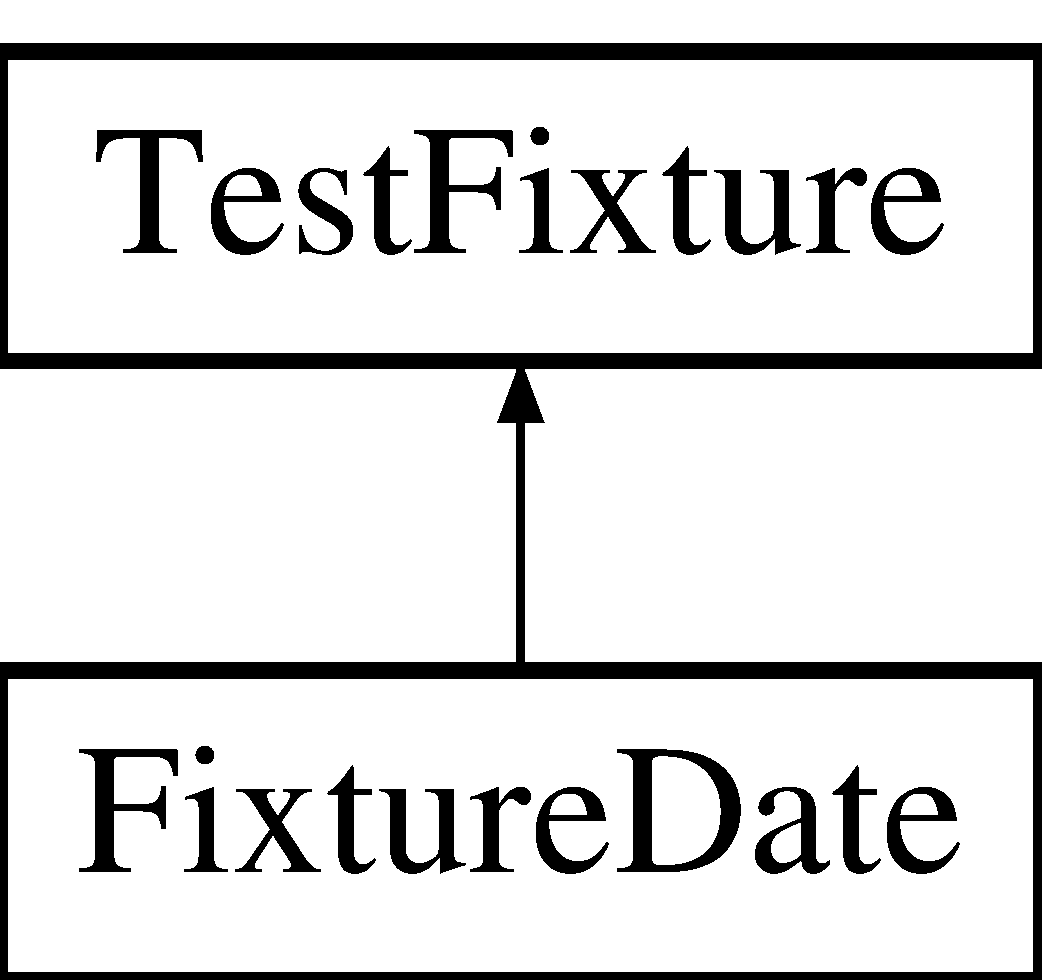
\includegraphics[height=2.000000cm]{classFixtureDate}
\end{center}
\end{figure}
\subsection*{Public Member Functions}
\begin{DoxyCompactItemize}
\item 
\hypertarget{classFixtureDate_a1f8d25cf20798bb3fa1f8a2360fbfc95}{{\bfseries C\-P\-P\-U\-N\-I\-T\-\_\-\-T\-E\-S\-T\-\_\-\-S\-U\-I\-T\-E} (\hyperlink{classFixtureDate}{Fixture\-Date})}\label{classFixtureDate_a1f8d25cf20798bb3fa1f8a2360fbfc95}

\item 
\hypertarget{classFixtureDate_ad5fca26ee7f19c0a418dfdf35484d9cd}{{\bfseries C\-P\-P\-U\-N\-I\-T\-\_\-\-T\-E\-S\-T} (\hyperlink{classFixtureDate_a69db7522ba1816b5d1629fdc801f5c37}{test\-Getter})}\label{classFixtureDate_ad5fca26ee7f19c0a418dfdf35484d9cd}

\item 
\hypertarget{classFixtureDate_a5e57aa30fe832610c0e3db885a6641b4}{{\bfseries C\-P\-P\-U\-N\-I\-T\-\_\-\-T\-E\-S\-T} (\hyperlink{classFixtureDate_a27c1d669174d0d6f8bf01e99c400e554}{test\-Setter})}\label{classFixtureDate_a5e57aa30fe832610c0e3db885a6641b4}

\item 
\hypertarget{classFixtureDate_a6feff25be84a29f329c3aaff2ff8182e}{{\bfseries C\-P\-P\-U\-N\-I\-T\-\_\-\-T\-E\-S\-T} (\hyperlink{classFixtureDate_a6c2ace09a60cf9f7d152c76e08f3fdbb}{test\-Para\-Constructor})}\label{classFixtureDate_a6feff25be84a29f329c3aaff2ff8182e}

\item 
\hypertarget{classFixtureDate_a09f76d326d06856b08e00f07246748b0}{{\bfseries C\-P\-P\-U\-N\-I\-T\-\_\-\-T\-E\-S\-T} (\hyperlink{classFixtureDate_a0d9371ca2466805d1701c9d0379017fd}{test\-Copy\-Constructor})}\label{classFixtureDate_a09f76d326d06856b08e00f07246748b0}

\item 
\hypertarget{classFixtureDate_acc8e5e32f61ad3962d5566c4780b9d01}{{\bfseries C\-P\-P\-U\-N\-I\-T\-\_\-\-T\-E\-S\-T} (\hyperlink{classFixtureDate_a15aae4ab5d11e2fee6e6094516536758}{test\-Next\-Date})}\label{classFixtureDate_acc8e5e32f61ad3962d5566c4780b9d01}

\item 
\hypertarget{classFixtureDate_ace0bc57449f553d3b8aa27cca0d40f3c}{{\bfseries C\-P\-P\-U\-N\-I\-T\-\_\-\-T\-E\-S\-T} (\hyperlink{classFixtureDate_a5877b14d8baa16bcb14e8d120195cefe}{test\-Is\-Valid})}\label{classFixtureDate_ace0bc57449f553d3b8aa27cca0d40f3c}

\item 
\hypertarget{classFixtureDate_ad3323f49f5e808d1e8a9922e24200374}{{\bfseries C\-P\-P\-U\-N\-I\-T\-\_\-\-T\-E\-S\-T} (\hyperlink{classFixtureDate_a94adf608fc780f68e18d7d88afad7e72}{test\-Equivalent})}\label{classFixtureDate_ad3323f49f5e808d1e8a9922e24200374}

\item 
\hypertarget{classFixtureDate_a99e62f3e9b12ebff1f18b0867ac65264}{{\bfseries C\-P\-P\-U\-N\-I\-T\-\_\-\-T\-E\-S\-T\-\_\-\-S\-U\-I\-T\-E\-\_\-\-E\-N\-D} ()}\label{classFixtureDate_a99e62f3e9b12ebff1f18b0867ac65264}

\item 
\hypertarget{classFixtureDate_a0cd645e7ffe8a60024c638b3fda44cea}{void {\bfseries set\-Up} ()}\label{classFixtureDate_a0cd645e7ffe8a60024c638b3fda44cea}

\item 
\hypertarget{classFixtureDate_a0a11c440cac2bb2298743688d03afdb3}{void {\bfseries tear\-Down} ()}\label{classFixtureDate_a0a11c440cac2bb2298743688d03afdb3}

\item 
void \hyperlink{classFixtureDate_a69db7522ba1816b5d1629fdc801f5c37}{test\-Getter} ()
\item 
void \hyperlink{classFixtureDate_a27c1d669174d0d6f8bf01e99c400e554}{test\-Setter} ()
\item 
void \hyperlink{classFixtureDate_a6c2ace09a60cf9f7d152c76e08f3fdbb}{test\-Para\-Constructor} ()
\item 
void \hyperlink{classFixtureDate_a0d9371ca2466805d1701c9d0379017fd}{test\-Copy\-Constructor} ()
\item 
void \hyperlink{classFixtureDate_a15aae4ab5d11e2fee6e6094516536758}{test\-Next\-Date} ()
\item 
void \hyperlink{classFixtureDate_a5877b14d8baa16bcb14e8d120195cefe}{test\-Is\-Valid} ()
\item 
void \hyperlink{classFixtureDate_a94adf608fc780f68e18d7d88afad7e72}{test\-Equivalent} ()
\end{DoxyCompactItemize}
\subsection*{Private Attributes}
\begin{DoxyCompactItemize}
\item 
\hypertarget{classFixtureDate_ae28deaac398bd33ee5d48c041442d9a0}{\hyperlink{classDate}{Date} $\ast$ {\bfseries dt}}\label{classFixtureDate_ae28deaac398bd33ee5d48c041442d9a0}

\end{DoxyCompactItemize}


\subsection{Member Function Documentation}
\hypertarget{classFixtureDate_a0d9371ca2466805d1701c9d0379017fd}{\index{Fixture\-Date@{Fixture\-Date}!test\-Copy\-Constructor@{test\-Copy\-Constructor}}
\index{test\-Copy\-Constructor@{test\-Copy\-Constructor}!FixtureDate@{Fixture\-Date}}
\subsubsection[{test\-Copy\-Constructor}]{\setlength{\rightskip}{0pt plus 5cm}void Fixture\-Date\-::test\-Copy\-Constructor (
\begin{DoxyParamCaption}
{}
\end{DoxyParamCaption}
)\hspace{0.3cm}{\ttfamily [inline]}}}\label{classFixtureDate_a0d9371ca2466805d1701c9d0379017fd}
Test for \hyperlink{classDate_a2233b93eaed1626e957435cedfc511de}{Date\-::\-Date(const Date\& dt)} \hypertarget{classFixtureDate_a94adf608fc780f68e18d7d88afad7e72}{\index{Fixture\-Date@{Fixture\-Date}!test\-Equivalent@{test\-Equivalent}}
\index{test\-Equivalent@{test\-Equivalent}!FixtureDate@{Fixture\-Date}}
\subsubsection[{test\-Equivalent}]{\setlength{\rightskip}{0pt plus 5cm}void Fixture\-Date\-::test\-Equivalent (
\begin{DoxyParamCaption}
{}
\end{DoxyParamCaption}
)\hspace{0.3cm}{\ttfamily [inline]}}}\label{classFixtureDate_a94adf608fc780f68e18d7d88afad7e72}
Test for equivalent check

Test case 1\-: 20150201==20150201 Test case 2\-: 20150202!=20150201 \hypertarget{classFixtureDate_a69db7522ba1816b5d1629fdc801f5c37}{\index{Fixture\-Date@{Fixture\-Date}!test\-Getter@{test\-Getter}}
\index{test\-Getter@{test\-Getter}!FixtureDate@{Fixture\-Date}}
\subsubsection[{test\-Getter}]{\setlength{\rightskip}{0pt plus 5cm}void Fixture\-Date\-::test\-Getter (
\begin{DoxyParamCaption}
{}
\end{DoxyParamCaption}
)\hspace{0.3cm}{\ttfamily [inline]}}}\label{classFixtureDate_a69db7522ba1816b5d1629fdc801f5c37}
Test for Date\-::get\-Date()

Default date is 20150301 \hypertarget{classFixtureDate_a5877b14d8baa16bcb14e8d120195cefe}{\index{Fixture\-Date@{Fixture\-Date}!test\-Is\-Valid@{test\-Is\-Valid}}
\index{test\-Is\-Valid@{test\-Is\-Valid}!FixtureDate@{Fixture\-Date}}
\subsubsection[{test\-Is\-Valid}]{\setlength{\rightskip}{0pt plus 5cm}void Fixture\-Date\-::test\-Is\-Valid (
\begin{DoxyParamCaption}
{}
\end{DoxyParamCaption}
)\hspace{0.3cm}{\ttfamily [inline]}}}\label{classFixtureDate_a5877b14d8baa16bcb14e8d120195cefe}
Test for \hyperlink{classDate_a7d9aaa9db591413e21c8b85fdae130ad}{Date\-::is\-Valid()}

Test case 1\-: 20150229(invalid)-\/$>$20150301 Test case 2\-: 20160229(valid)-\/$>$20160229 Test case 3\-: 20151930(invalid)-\/$>$20150301 \hypertarget{classFixtureDate_a15aae4ab5d11e2fee6e6094516536758}{\index{Fixture\-Date@{Fixture\-Date}!test\-Next\-Date@{test\-Next\-Date}}
\index{test\-Next\-Date@{test\-Next\-Date}!FixtureDate@{Fixture\-Date}}
\subsubsection[{test\-Next\-Date}]{\setlength{\rightskip}{0pt plus 5cm}void Fixture\-Date\-::test\-Next\-Date (
\begin{DoxyParamCaption}
{}
\end{DoxyParamCaption}
)\hspace{0.3cm}{\ttfamily [inline]}}}\label{classFixtureDate_a15aae4ab5d11e2fee6e6094516536758}
Test for \hyperlink{classDate_a689d13b5e5882068308b02073e1ed321}{Date\-::next\-Date()}

Test case 1\-: 20150228-\/$>$20150301 Test case 2\-: 20160228-\/$>$20160229 Test case 3\-: 20150930-\/$>$20151001 Test case 4\-: 20151215-\/$>$20151216 \hypertarget{classFixtureDate_a6c2ace09a60cf9f7d152c76e08f3fdbb}{\index{Fixture\-Date@{Fixture\-Date}!test\-Para\-Constructor@{test\-Para\-Constructor}}
\index{test\-Para\-Constructor@{test\-Para\-Constructor}!FixtureDate@{Fixture\-Date}}
\subsubsection[{test\-Para\-Constructor}]{\setlength{\rightskip}{0pt plus 5cm}void Fixture\-Date\-::test\-Para\-Constructor (
\begin{DoxyParamCaption}
{}
\end{DoxyParamCaption}
)\hspace{0.3cm}{\ttfamily [inline]}}}\label{classFixtureDate_a6c2ace09a60cf9f7d152c76e08f3fdbb}
Test for \hyperlink{classDate_a86d5d0d04d211f5fa077386de1ce7f19}{Date\-::\-Date(int d)} \hypertarget{classFixtureDate_a27c1d669174d0d6f8bf01e99c400e554}{\index{Fixture\-Date@{Fixture\-Date}!test\-Setter@{test\-Setter}}
\index{test\-Setter@{test\-Setter}!FixtureDate@{Fixture\-Date}}
\subsubsection[{test\-Setter}]{\setlength{\rightskip}{0pt plus 5cm}void Fixture\-Date\-::test\-Setter (
\begin{DoxyParamCaption}
{}
\end{DoxyParamCaption}
)\hspace{0.3cm}{\ttfamily [inline]}}}\label{classFixtureDate_a27c1d669174d0d6f8bf01e99c400e554}
Test for Date\-::set\-Date(int d) 

The documentation for this class was generated from the following file\-:\begin{DoxyCompactItemize}
\item 
\hyperlink{FixtureDate_8h}{Fixture\-Date.\-h}\end{DoxyCompactItemize}

\hypertarget{classFixtureState}{\section{Fixture\-State Class Reference}
\label{classFixtureState}\index{Fixture\-State@{Fixture\-State}}
}
Inheritance diagram for Fixture\-State\-:\begin{figure}[H]
\begin{center}
\leavevmode
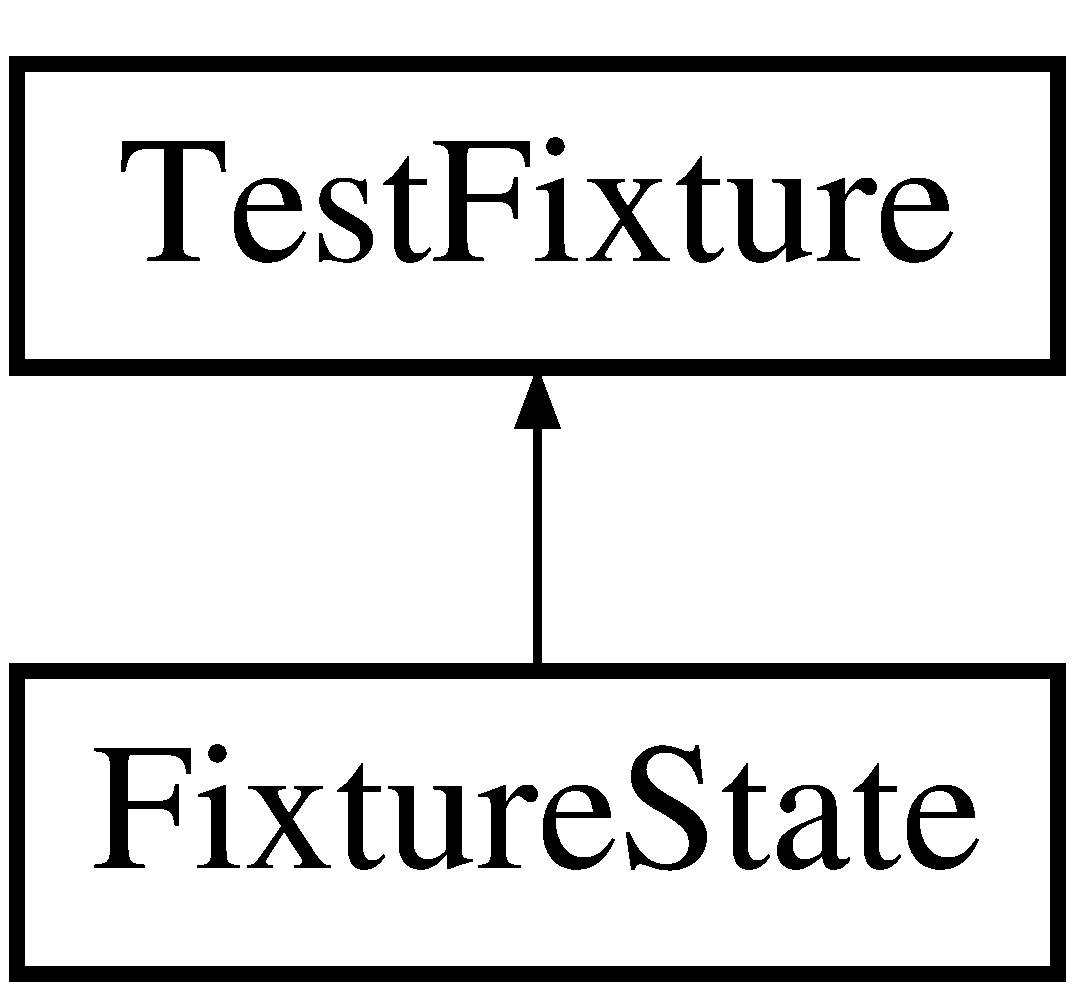
\includegraphics[height=2.000000cm]{classFixtureState}
\end{center}
\end{figure}
\subsection*{Public Member Functions}
\begin{DoxyCompactItemize}
\item 
\hypertarget{classFixtureState_a22fb7720f4a564d437668118be93cf97}{{\bfseries C\-P\-P\-U\-N\-I\-T\-\_\-\-T\-E\-S\-T\-\_\-\-S\-U\-I\-T\-E} (\hyperlink{classFixtureState}{Fixture\-State})}\label{classFixtureState_a22fb7720f4a564d437668118be93cf97}

\item 
\hypertarget{classFixtureState_a1ccf1873828a5015c45ada8901521e23}{{\bfseries C\-P\-P\-U\-N\-I\-T\-\_\-\-T\-E\-S\-T} (\hyperlink{classFixtureState_adebc4786a79503e8043e7656b685553d}{test\-Date\-Getter})}\label{classFixtureState_a1ccf1873828a5015c45ada8901521e23}

\item 
\hypertarget{classFixtureState_ac230d800bc3ee6d805d9a1cbff95a154}{{\bfseries C\-P\-P\-U\-N\-I\-T\-\_\-\-T\-E\-S\-T} (\hyperlink{classFixtureState_a78b6da6dc98770d6ba888c505abfbe75}{test\-Date\-Setter})}\label{classFixtureState_ac230d800bc3ee6d805d9a1cbff95a154}

\item 
\hypertarget{classFixtureState_af9402cb92dc50b4efd68dbed84242ebe}{{\bfseries C\-P\-P\-U\-N\-I\-T\-\_\-\-T\-E\-S\-T} (\hyperlink{classFixtureState_a483306b02bf3727eda3cbc852e2bf782}{test\-Content\-Getter})}\label{classFixtureState_af9402cb92dc50b4efd68dbed84242ebe}

\item 
\hypertarget{classFixtureState_a8502029a4eaceb97498bc4620056449b}{{\bfseries C\-P\-P\-U\-N\-I\-T\-\_\-\-T\-E\-S\-T} (\hyperlink{classFixtureState_ade2b801626053e1a466932100385728a}{test\-Content\-Setter})}\label{classFixtureState_a8502029a4eaceb97498bc4620056449b}

\item 
\hypertarget{classFixtureState_a2f6b20d53e1458e9b96152716d869f8e}{{\bfseries C\-P\-P\-U\-N\-I\-T\-\_\-\-T\-E\-S\-T} (\hyperlink{classFixtureState_a9ef71fada62e876202304729bd936f25}{test\-Para\-Constructor})}\label{classFixtureState_a2f6b20d53e1458e9b96152716d869f8e}

\item 
\hypertarget{classFixtureState_a64c6570528a0d653f49da97b08b0b51c}{{\bfseries C\-P\-P\-U\-N\-I\-T\-\_\-\-T\-E\-S\-T} (\hyperlink{classFixtureState_aad72e91e1c12f29e9a272e06ee9c8bec}{test\-Copy\-Constructor})}\label{classFixtureState_a64c6570528a0d653f49da97b08b0b51c}

\item 
\hypertarget{classFixtureState_a0158583e0e3ea8facc087e6b19ecc709}{{\bfseries C\-P\-P\-U\-N\-I\-T\-\_\-\-T\-E\-S\-T} (\hyperlink{classFixtureState_a74e4df88858f1d5cae700eb0b891d790}{test\-Content\-Merge})}\label{classFixtureState_a0158583e0e3ea8facc087e6b19ecc709}

\item 
\hypertarget{classFixtureState_af28e12e2f700210a55600ec386308a43}{{\bfseries C\-P\-P\-U\-N\-I\-T\-\_\-\-T\-E\-S\-T} (\hyperlink{classFixtureState_aca99d95e2e771d5a7f89de3d247576da}{test\-State\-Merge})}\label{classFixtureState_af28e12e2f700210a55600ec386308a43}

\item 
\hypertarget{classFixtureState_a9262f63cbc9b4b88cce1a51938f893ab}{{\bfseries C\-P\-P\-U\-N\-I\-T\-\_\-\-T\-E\-S\-T\-\_\-\-S\-U\-I\-T\-E\-\_\-\-E\-N\-D} ()}\label{classFixtureState_a9262f63cbc9b4b88cce1a51938f893ab}

\item 
\hypertarget{classFixtureState_a14721f818a412449fb768a06ecd441f9}{void {\bfseries set\-Up} ()}\label{classFixtureState_a14721f818a412449fb768a06ecd441f9}

\item 
\hypertarget{classFixtureState_adfde2705e5fed8ca1ec95e670c07cf42}{void {\bfseries tear\-Down} ()}\label{classFixtureState_adfde2705e5fed8ca1ec95e670c07cf42}

\item 
void \hyperlink{classFixtureState_a78b6da6dc98770d6ba888c505abfbe75}{test\-Date\-Setter} ()
\item 
void \hyperlink{classFixtureState_adebc4786a79503e8043e7656b685553d}{test\-Date\-Getter} ()
\item 
void \hyperlink{classFixtureState_ade2b801626053e1a466932100385728a}{test\-Content\-Setter} ()
\item 
void \hyperlink{classFixtureState_a483306b02bf3727eda3cbc852e2bf782}{test\-Content\-Getter} ()
\item 
void \hyperlink{classFixtureState_a9ef71fada62e876202304729bd936f25}{test\-Para\-Constructor} ()
\item 
void \hyperlink{classFixtureState_aad72e91e1c12f29e9a272e06ee9c8bec}{test\-Copy\-Constructor} ()
\item 
void \hyperlink{classFixtureState_a74e4df88858f1d5cae700eb0b891d790}{test\-Content\-Merge} ()
\item 
void \hyperlink{classFixtureState_aca99d95e2e771d5a7f89de3d247576da}{test\-State\-Merge} ()
\end{DoxyCompactItemize}
\subsection*{Private Attributes}
\begin{DoxyCompactItemize}
\item 
\hypertarget{classFixtureState_aebd5943051db19e13224f8eac5c39fee}{\hyperlink{classState}{State} $\ast$ {\bfseries st}}\label{classFixtureState_aebd5943051db19e13224f8eac5c39fee}

\end{DoxyCompactItemize}


\subsection{Member Function Documentation}
\hypertarget{classFixtureState_a483306b02bf3727eda3cbc852e2bf782}{\index{Fixture\-State@{Fixture\-State}!test\-Content\-Getter@{test\-Content\-Getter}}
\index{test\-Content\-Getter@{test\-Content\-Getter}!FixtureState@{Fixture\-State}}
\subsubsection[{test\-Content\-Getter}]{\setlength{\rightskip}{0pt plus 5cm}void Fixture\-State\-::test\-Content\-Getter (
\begin{DoxyParamCaption}
{}
\end{DoxyParamCaption}
)\hspace{0.3cm}{\ttfamily [inline]}}}\label{classFixtureState_a483306b02bf3727eda3cbc852e2bf782}
Test for \hyperlink{classState_a8718dda1c97b278380d14f686d85116f}{State\-::get\-Content()} \hypertarget{classFixtureState_a74e4df88858f1d5cae700eb0b891d790}{\index{Fixture\-State@{Fixture\-State}!test\-Content\-Merge@{test\-Content\-Merge}}
\index{test\-Content\-Merge@{test\-Content\-Merge}!FixtureState@{Fixture\-State}}
\subsubsection[{test\-Content\-Merge}]{\setlength{\rightskip}{0pt plus 5cm}void Fixture\-State\-::test\-Content\-Merge (
\begin{DoxyParamCaption}
{}
\end{DoxyParamCaption}
)\hspace{0.3cm}{\ttfamily [inline]}}}\label{classFixtureState_a74e4df88858f1d5cae700eb0b891d790}
Test for \hyperlink{classState_a61aee26c30eed819471404242b392518}{State\-::merge(std\-::string s)} \hypertarget{classFixtureState_ade2b801626053e1a466932100385728a}{\index{Fixture\-State@{Fixture\-State}!test\-Content\-Setter@{test\-Content\-Setter}}
\index{test\-Content\-Setter@{test\-Content\-Setter}!FixtureState@{Fixture\-State}}
\subsubsection[{test\-Content\-Setter}]{\setlength{\rightskip}{0pt plus 5cm}void Fixture\-State\-::test\-Content\-Setter (
\begin{DoxyParamCaption}
{}
\end{DoxyParamCaption}
)\hspace{0.3cm}{\ttfamily [inline]}}}\label{classFixtureState_ade2b801626053e1a466932100385728a}
Test for \hyperlink{classState_aa8d9dbc292caef3a38ebd7460a4d00a5}{State\-::set\-Content(std\-::string s)} \hypertarget{classFixtureState_aad72e91e1c12f29e9a272e06ee9c8bec}{\index{Fixture\-State@{Fixture\-State}!test\-Copy\-Constructor@{test\-Copy\-Constructor}}
\index{test\-Copy\-Constructor@{test\-Copy\-Constructor}!FixtureState@{Fixture\-State}}
\subsubsection[{test\-Copy\-Constructor}]{\setlength{\rightskip}{0pt plus 5cm}void Fixture\-State\-::test\-Copy\-Constructor (
\begin{DoxyParamCaption}
{}
\end{DoxyParamCaption}
)\hspace{0.3cm}{\ttfamily [inline]}}}\label{classFixtureState_aad72e91e1c12f29e9a272e06ee9c8bec}
Test for \hyperlink{classState_a893ddf069c68f0b3b0b019f56787f6c5}{State\-::\-State(const State\& st)} \hypertarget{classFixtureState_adebc4786a79503e8043e7656b685553d}{\index{Fixture\-State@{Fixture\-State}!test\-Date\-Getter@{test\-Date\-Getter}}
\index{test\-Date\-Getter@{test\-Date\-Getter}!FixtureState@{Fixture\-State}}
\subsubsection[{test\-Date\-Getter}]{\setlength{\rightskip}{0pt plus 5cm}void Fixture\-State\-::test\-Date\-Getter (
\begin{DoxyParamCaption}
{}
\end{DoxyParamCaption}
)\hspace{0.3cm}{\ttfamily [inline]}}}\label{classFixtureState_adebc4786a79503e8043e7656b685553d}
Test for \hyperlink{classState_a3664da3a20958900365cdd76658e6d4a}{State\-::get\-Date()} \hypertarget{classFixtureState_a78b6da6dc98770d6ba888c505abfbe75}{\index{Fixture\-State@{Fixture\-State}!test\-Date\-Setter@{test\-Date\-Setter}}
\index{test\-Date\-Setter@{test\-Date\-Setter}!FixtureState@{Fixture\-State}}
\subsubsection[{test\-Date\-Setter}]{\setlength{\rightskip}{0pt plus 5cm}void Fixture\-State\-::test\-Date\-Setter (
\begin{DoxyParamCaption}
{}
\end{DoxyParamCaption}
)\hspace{0.3cm}{\ttfamily [inline]}}}\label{classFixtureState_a78b6da6dc98770d6ba888c505abfbe75}
Test for Sate\-::set\-Date(const Date\& dt) \hypertarget{classFixtureState_a9ef71fada62e876202304729bd936f25}{\index{Fixture\-State@{Fixture\-State}!test\-Para\-Constructor@{test\-Para\-Constructor}}
\index{test\-Para\-Constructor@{test\-Para\-Constructor}!FixtureState@{Fixture\-State}}
\subsubsection[{test\-Para\-Constructor}]{\setlength{\rightskip}{0pt plus 5cm}void Fixture\-State\-::test\-Para\-Constructor (
\begin{DoxyParamCaption}
{}
\end{DoxyParamCaption}
)\hspace{0.3cm}{\ttfamily [inline]}}}\label{classFixtureState_a9ef71fada62e876202304729bd936f25}
Test for \hyperlink{classState_acc328bb9bcea278074ba7dd8f4fd669d}{State\-::\-State(std\-::string s, const Date\& dt)} \hypertarget{classFixtureState_aca99d95e2e771d5a7f89de3d247576da}{\index{Fixture\-State@{Fixture\-State}!test\-State\-Merge@{test\-State\-Merge}}
\index{test\-State\-Merge@{test\-State\-Merge}!FixtureState@{Fixture\-State}}
\subsubsection[{test\-State\-Merge}]{\setlength{\rightskip}{0pt plus 5cm}void Fixture\-State\-::test\-State\-Merge (
\begin{DoxyParamCaption}
{}
\end{DoxyParamCaption}
)\hspace{0.3cm}{\ttfamily [inline]}}}\label{classFixtureState_aca99d95e2e771d5a7f89de3d247576da}
Test for \hyperlink{classState_aa8e95f73956f3ffbea5e1d5076df32e8}{State\-::merge(\-State st)} 

The documentation for this class was generated from the following file\-:\begin{DoxyCompactItemize}
\item 
\hyperlink{FixtureState_8h}{Fixture\-State.\-h}\end{DoxyCompactItemize}

\hypertarget{classFixtureTask}{\section{Fixture\-Task Class Reference}
\label{classFixtureTask}\index{Fixture\-Task@{Fixture\-Task}}
}
Inheritance diagram for Fixture\-Task\-:\begin{figure}[H]
\begin{center}
\leavevmode
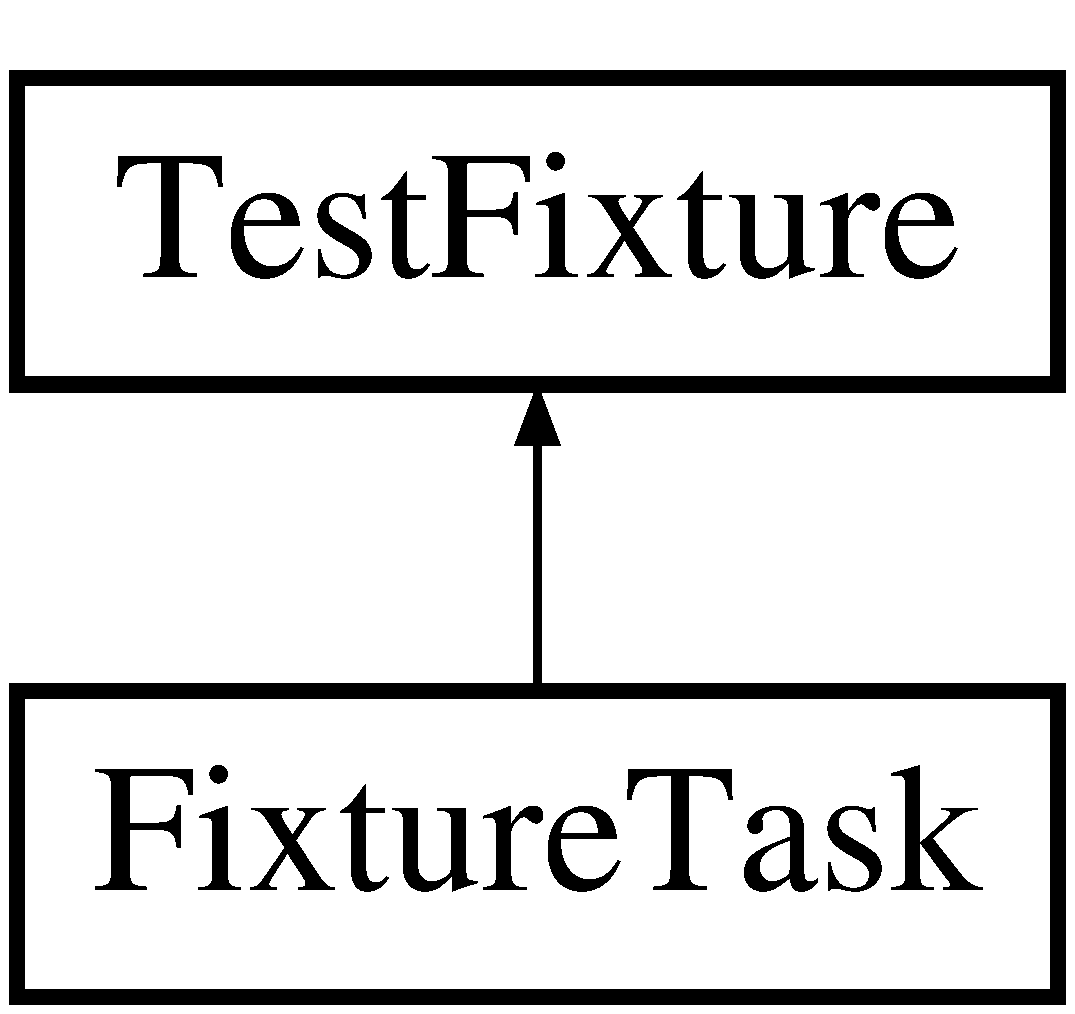
\includegraphics[height=2.000000cm]{classFixtureTask}
\end{center}
\end{figure}
\subsection*{Public Member Functions}
\begin{DoxyCompactItemize}
\item 
\hypertarget{classFixtureTask_a5f0ed2a3a14d7a73cb7f4947977e679d}{{\bfseries C\-P\-P\-U\-N\-I\-T\-\_\-\-T\-E\-S\-T\-\_\-\-S\-U\-I\-T\-E} (\hyperlink{classFixtureTask}{Fixture\-Task})}\label{classFixtureTask_a5f0ed2a3a14d7a73cb7f4947977e679d}

\item 
\hypertarget{classFixtureTask_a2a72e34545ad8a92645e517622d46535}{{\bfseries C\-P\-P\-U\-N\-I\-T\-\_\-\-T\-E\-S\-T} (\hyperlink{classFixtureTask_aa6c4e049025fb8fec20e3e4f01f11af9}{test\-Task\-Name\-Getter})}\label{classFixtureTask_a2a72e34545ad8a92645e517622d46535}

\item 
\hypertarget{classFixtureTask_a32fa0554db694ef965b8a76f54efc632}{{\bfseries C\-P\-P\-U\-N\-I\-T\-\_\-\-T\-E\-S\-T} (\hyperlink{classFixtureTask_a7ca68394afb06b5ed6ee577bf41b97d5}{test\-Task\-Name\-Setter})}\label{classFixtureTask_a32fa0554db694ef965b8a76f54efc632}

\item 
\hypertarget{classFixtureTask_a66e558daf1fee5703b59c29da90230e4}{{\bfseries C\-P\-P\-U\-N\-I\-T\-\_\-\-T\-E\-S\-T} (\hyperlink{classFixtureTask_ab1f178b4ebcd6d2f81896e3bbda6e40b}{test\-Status\-Getter})}\label{classFixtureTask_a66e558daf1fee5703b59c29da90230e4}

\item 
\hypertarget{classFixtureTask_a381580da60309dfb883cb857da3979fe}{{\bfseries C\-P\-P\-U\-N\-I\-T\-\_\-\-T\-E\-S\-T} (\hyperlink{classFixtureTask_a6f293436620532dbeb744b4a1e49710e}{test\-Status\-Setter})}\label{classFixtureTask_a381580da60309dfb883cb857da3979fe}

\item 
\hypertarget{classFixtureTask_a22963e7f2ec438696a7e2da17a5e2bf6}{{\bfseries C\-P\-P\-U\-N\-I\-T\-\_\-\-T\-E\-S\-T} (\hyperlink{classFixtureTask_aef7e5a1e9e70606248de77b6aa5dcdc7}{test\-State\-Getter})}\label{classFixtureTask_a22963e7f2ec438696a7e2da17a5e2bf6}

\item 
\hypertarget{classFixtureTask_afef20f5e6367eba0dafd1cd07a406501}{{\bfseries C\-P\-P\-U\-N\-I\-T\-\_\-\-T\-E\-S\-T} (\hyperlink{classFixtureTask_a0a1655fc0353b5aaa147f16724c17e46}{test\-State\-Setter})}\label{classFixtureTask_afef20f5e6367eba0dafd1cd07a406501}

\item 
\hypertarget{classFixtureTask_a0b9535a87a3311a4cede7f925a9b0005}{{\bfseries C\-P\-P\-U\-N\-I\-T\-\_\-\-T\-E\-S\-T} (\hyperlink{classFixtureTask_ab02c2f1ac774c37fbaf8bf01a95d765f}{test\-Para\-Constructor})}\label{classFixtureTask_a0b9535a87a3311a4cede7f925a9b0005}

\item 
\hypertarget{classFixtureTask_a4cd66ea3ae59eea1e79fe21e68bc55e2}{{\bfseries C\-P\-P\-U\-N\-I\-T\-\_\-\-T\-E\-S\-T} (\hyperlink{classFixtureTask_a1cdcb138e1c95b84d03959310064c401}{test\-Copy\-Constructor})}\label{classFixtureTask_a4cd66ea3ae59eea1e79fe21e68bc55e2}

\item 
\hypertarget{classFixtureTask_ae952ff2105ae208a4f346a2e1f3f88f8}{{\bfseries C\-P\-P\-U\-N\-I\-T\-\_\-\-T\-E\-S\-T\-\_\-\-S\-U\-I\-T\-E\-\_\-\-E\-N\-D} ()}\label{classFixtureTask_ae952ff2105ae208a4f346a2e1f3f88f8}

\item 
\hypertarget{classFixtureTask_a6842ba348d475991610fc4988d5013f8}{void {\bfseries set\-Up} ()}\label{classFixtureTask_a6842ba348d475991610fc4988d5013f8}

\item 
\hypertarget{classFixtureTask_ae595b1036bfc302569e7b7359eba64af}{void {\bfseries tear\-Down} ()}\label{classFixtureTask_ae595b1036bfc302569e7b7359eba64af}

\item 
void \hyperlink{classFixtureTask_aa6c4e049025fb8fec20e3e4f01f11af9}{test\-Task\-Name\-Getter} ()
\item 
void \hyperlink{classFixtureTask_a7ca68394afb06b5ed6ee577bf41b97d5}{test\-Task\-Name\-Setter} ()
\item 
void \hyperlink{classFixtureTask_ab1f178b4ebcd6d2f81896e3bbda6e40b}{test\-Status\-Getter} ()
\item 
void \hyperlink{classFixtureTask_a6f293436620532dbeb744b4a1e49710e}{test\-Status\-Setter} ()
\item 
void \hyperlink{classFixtureTask_aef7e5a1e9e70606248de77b6aa5dcdc7}{test\-State\-Getter} ()
\item 
void \hyperlink{classFixtureTask_a0a1655fc0353b5aaa147f16724c17e46}{test\-State\-Setter} ()
\item 
void \hyperlink{classFixtureTask_ab02c2f1ac774c37fbaf8bf01a95d765f}{test\-Para\-Constructor} ()
\item 
void \hyperlink{classFixtureTask_a1cdcb138e1c95b84d03959310064c401}{test\-Copy\-Constructor} ()
\end{DoxyCompactItemize}
\subsection*{Private Attributes}
\begin{DoxyCompactItemize}
\item 
\hypertarget{classFixtureTask_af5824b2aa836ff4f5269686970e2eaf2}{\hyperlink{classTask}{Task} $\ast$ {\bfseries t}}\label{classFixtureTask_af5824b2aa836ff4f5269686970e2eaf2}

\end{DoxyCompactItemize}


\subsection{Member Function Documentation}
\hypertarget{classFixtureTask_a1cdcb138e1c95b84d03959310064c401}{\index{Fixture\-Task@{Fixture\-Task}!test\-Copy\-Constructor@{test\-Copy\-Constructor}}
\index{test\-Copy\-Constructor@{test\-Copy\-Constructor}!FixtureTask@{Fixture\-Task}}
\subsubsection[{test\-Copy\-Constructor}]{\setlength{\rightskip}{0pt plus 5cm}void Fixture\-Task\-::test\-Copy\-Constructor (
\begin{DoxyParamCaption}
{}
\end{DoxyParamCaption}
)\hspace{0.3cm}{\ttfamily [inline]}}}\label{classFixtureTask_a1cdcb138e1c95b84d03959310064c401}
Test for Task\-::test\-Copy\-Constructor(const Task\&) \hypertarget{classFixtureTask_ab02c2f1ac774c37fbaf8bf01a95d765f}{\index{Fixture\-Task@{Fixture\-Task}!test\-Para\-Constructor@{test\-Para\-Constructor}}
\index{test\-Para\-Constructor@{test\-Para\-Constructor}!FixtureTask@{Fixture\-Task}}
\subsubsection[{test\-Para\-Constructor}]{\setlength{\rightskip}{0pt plus 5cm}void Fixture\-Task\-::test\-Para\-Constructor (
\begin{DoxyParamCaption}
{}
\end{DoxyParamCaption}
)\hspace{0.3cm}{\ttfamily [inline]}}}\label{classFixtureTask_ab02c2f1ac774c37fbaf8bf01a95d765f}
Test for Task\-::test\-Para\-Constructor \hypertarget{classFixtureTask_aef7e5a1e9e70606248de77b6aa5dcdc7}{\index{Fixture\-Task@{Fixture\-Task}!test\-State\-Getter@{test\-State\-Getter}}
\index{test\-State\-Getter@{test\-State\-Getter}!FixtureTask@{Fixture\-Task}}
\subsubsection[{test\-State\-Getter}]{\setlength{\rightskip}{0pt plus 5cm}void Fixture\-Task\-::test\-State\-Getter (
\begin{DoxyParamCaption}
{}
\end{DoxyParamCaption}
)\hspace{0.3cm}{\ttfamily [inline]}}}\label{classFixtureTask_aef7e5a1e9e70606248de77b6aa5dcdc7}
Test for Task\-::test\-Status\-Getter() \hypertarget{classFixtureTask_a0a1655fc0353b5aaa147f16724c17e46}{\index{Fixture\-Task@{Fixture\-Task}!test\-State\-Setter@{test\-State\-Setter}}
\index{test\-State\-Setter@{test\-State\-Setter}!FixtureTask@{Fixture\-Task}}
\subsubsection[{test\-State\-Setter}]{\setlength{\rightskip}{0pt plus 5cm}void Fixture\-Task\-::test\-State\-Setter (
\begin{DoxyParamCaption}
{}
\end{DoxyParamCaption}
)\hspace{0.3cm}{\ttfamily [inline]}}}\label{classFixtureTask_a0a1655fc0353b5aaa147f16724c17e46}
Test for Task\-::test\-Status\-Setter(const\& vector$<$state$>$) \hypertarget{classFixtureTask_ab1f178b4ebcd6d2f81896e3bbda6e40b}{\index{Fixture\-Task@{Fixture\-Task}!test\-Status\-Getter@{test\-Status\-Getter}}
\index{test\-Status\-Getter@{test\-Status\-Getter}!FixtureTask@{Fixture\-Task}}
\subsubsection[{test\-Status\-Getter}]{\setlength{\rightskip}{0pt plus 5cm}void Fixture\-Task\-::test\-Status\-Getter (
\begin{DoxyParamCaption}
{}
\end{DoxyParamCaption}
)\hspace{0.3cm}{\ttfamily [inline]}}}\label{classFixtureTask_ab1f178b4ebcd6d2f81896e3bbda6e40b}
Test for Task\-::test\-Status\-Getter() \hypertarget{classFixtureTask_a6f293436620532dbeb744b4a1e49710e}{\index{Fixture\-Task@{Fixture\-Task}!test\-Status\-Setter@{test\-Status\-Setter}}
\index{test\-Status\-Setter@{test\-Status\-Setter}!FixtureTask@{Fixture\-Task}}
\subsubsection[{test\-Status\-Setter}]{\setlength{\rightskip}{0pt plus 5cm}void Fixture\-Task\-::test\-Status\-Setter (
\begin{DoxyParamCaption}
{}
\end{DoxyParamCaption}
)\hspace{0.3cm}{\ttfamily [inline]}}}\label{classFixtureTask_a6f293436620532dbeb744b4a1e49710e}
Test for Task\-::test\-Status\-Setter(int) \hypertarget{classFixtureTask_aa6c4e049025fb8fec20e3e4f01f11af9}{\index{Fixture\-Task@{Fixture\-Task}!test\-Task\-Name\-Getter@{test\-Task\-Name\-Getter}}
\index{test\-Task\-Name\-Getter@{test\-Task\-Name\-Getter}!FixtureTask@{Fixture\-Task}}
\subsubsection[{test\-Task\-Name\-Getter}]{\setlength{\rightskip}{0pt plus 5cm}void Fixture\-Task\-::test\-Task\-Name\-Getter (
\begin{DoxyParamCaption}
{}
\end{DoxyParamCaption}
)\hspace{0.3cm}{\ttfamily [inline]}}}\label{classFixtureTask_aa6c4e049025fb8fec20e3e4f01f11af9}
Test for \hyperlink{classTask_abb5dae8b5244e54c7d5015b2e788d803}{Task\-::get\-Task\-Name()} \hypertarget{classFixtureTask_a7ca68394afb06b5ed6ee577bf41b97d5}{\index{Fixture\-Task@{Fixture\-Task}!test\-Task\-Name\-Setter@{test\-Task\-Name\-Setter}}
\index{test\-Task\-Name\-Setter@{test\-Task\-Name\-Setter}!FixtureTask@{Fixture\-Task}}
\subsubsection[{test\-Task\-Name\-Setter}]{\setlength{\rightskip}{0pt plus 5cm}void Fixture\-Task\-::test\-Task\-Name\-Setter (
\begin{DoxyParamCaption}
{}
\end{DoxyParamCaption}
)\hspace{0.3cm}{\ttfamily [inline]}}}\label{classFixtureTask_a7ca68394afb06b5ed6ee577bf41b97d5}
Test for Task\-::set\-Task\-Name(string) 

The documentation for this class was generated from the following file\-:\begin{DoxyCompactItemize}
\item 
\hyperlink{FixtureTask_8h}{Fixture\-Task.\-h}\end{DoxyCompactItemize}

\hypertarget{classState}{\section{State Class Reference}
\label{classState}\index{State@{State}}
}


\hyperlink{classState}{State} Class is used to record a progress of a task.  




{\ttfamily \#include $<$State.\-h$>$}

\subsection*{Public Member Functions}
\begin{DoxyCompactItemize}
\item 
\hyperlink{classState_ab91bb1dd5aa6260ab2a456581daf9ec2}{State} ()
\item 
\hyperlink{classState_acc328bb9bcea278074ba7dd8f4fd669d}{State} (std\-::string s, const \hyperlink{classDate}{Date} \&dt)
\item 
\hyperlink{classState_a893ddf069c68f0b3b0b019f56787f6c5}{State} (const \hyperlink{classState}{State} \&st)
\item 
\hyperlink{classState_afab438d92b90dc18d194dbd9c9c8bab3}{$\sim$\-State} ()
\item 
void \hyperlink{classState_ab13c5851bcdbbe40b8b56397aca753bc}{set\-Date} (const \hyperlink{classDate}{Date} \&dt)
\item 
\hyperlink{classDate}{Date} \hyperlink{classState_a3664da3a20958900365cdd76658e6d4a}{get\-Date} ()
\item 
void \hyperlink{classState_aa8d9dbc292caef3a38ebd7460a4d00a5}{set\-Content} (std\-::string s)
\item 
std\-::string \hyperlink{classState_a8718dda1c97b278380d14f686d85116f}{get\-Content} ()
\item 
void \hyperlink{classState_a61aee26c30eed819471404242b392518}{merge} (std\-::string s)
\item 
void \hyperlink{classState_aa8e95f73956f3ffbea5e1d5076df32e8}{merge} (\hyperlink{classState}{State} st)
\end{DoxyCompactItemize}
\subsection*{Private Attributes}
\begin{DoxyCompactItemize}
\item 
std\-::string \hyperlink{classState_a571e4d3107736dc2074ab985cff9ad20}{content}
\item 
\hyperlink{classDate}{Date} \hyperlink{classState_aa84f5430996a657c5658791b556fb8db}{date}
\end{DoxyCompactItemize}


\subsection{Detailed Description}
\hyperlink{classState}{State} Class is used to record a progress of a task. 

\hyperlink{classState}{State} Class records both progress detail and performing date. \hyperlink{classState}{State} Class also provides some basic operations related with a progress. 

\subsection{Constructor \& Destructor Documentation}
\hypertarget{classState_ab91bb1dd5aa6260ab2a456581daf9ec2}{\index{State@{State}!State@{State}}
\index{State@{State}!State@{State}}
\subsubsection[{State}]{\setlength{\rightskip}{0pt plus 5cm}State\-::\-State (
\begin{DoxyParamCaption}
{}
\end{DoxyParamCaption}
)}}\label{classState_ab91bb1dd5aa6260ab2a456581daf9ec2}
Default constructor \hypertarget{classState_acc328bb9bcea278074ba7dd8f4fd669d}{\index{State@{State}!State@{State}}
\index{State@{State}!State@{State}}
\subsubsection[{State}]{\setlength{\rightskip}{0pt plus 5cm}State\-::\-State (
\begin{DoxyParamCaption}
\item[{std\-::string}]{s, }
\item[{const {\bf Date} \&}]{dt}
\end{DoxyParamCaption}
)}}\label{classState_acc328bb9bcea278074ba7dd8f4fd669d}
Parameterized constructor 
\begin{DoxyParams}{Parameters}
{\em s} & string content for a progress \\
\hline
{\em dt} & a \hyperlink{classDate}{Date} object \\
\hline
\end{DoxyParams}
\hypertarget{classState_a893ddf069c68f0b3b0b019f56787f6c5}{\index{State@{State}!State@{State}}
\index{State@{State}!State@{State}}
\subsubsection[{State}]{\setlength{\rightskip}{0pt plus 5cm}State\-::\-State (
\begin{DoxyParamCaption}
\item[{const {\bf State} \&}]{st}
\end{DoxyParamCaption}
)}}\label{classState_a893ddf069c68f0b3b0b019f56787f6c5}
Copy constructor \hypertarget{classState_afab438d92b90dc18d194dbd9c9c8bab3}{\index{State@{State}!$\sim$\-State@{$\sim$\-State}}
\index{$\sim$\-State@{$\sim$\-State}!State@{State}}
\subsubsection[{$\sim$\-State}]{\setlength{\rightskip}{0pt plus 5cm}State\-::$\sim$\-State (
\begin{DoxyParamCaption}
{}
\end{DoxyParamCaption}
)}}\label{classState_afab438d92b90dc18d194dbd9c9c8bab3}
Destructor 

\subsection{Member Function Documentation}
\hypertarget{classState_a8718dda1c97b278380d14f686d85116f}{\index{State@{State}!get\-Content@{get\-Content}}
\index{get\-Content@{get\-Content}!State@{State}}
\subsubsection[{get\-Content}]{\setlength{\rightskip}{0pt plus 5cm}std\-::string State\-::get\-Content (
\begin{DoxyParamCaption}
{}
\end{DoxyParamCaption}
)}}\label{classState_a8718dda1c97b278380d14f686d85116f}
Getter for content \begin{DoxyReturn}{Returns}
A string with details from private content 
\end{DoxyReturn}
\hypertarget{classState_a3664da3a20958900365cdd76658e6d4a}{\index{State@{State}!get\-Date@{get\-Date}}
\index{get\-Date@{get\-Date}!State@{State}}
\subsubsection[{get\-Date}]{\setlength{\rightskip}{0pt plus 5cm}{\bf Date} State\-::get\-Date (
\begin{DoxyParamCaption}
{}
\end{DoxyParamCaption}
)}}\label{classState_a3664da3a20958900365cdd76658e6d4a}
Getter for date \begin{DoxyReturn}{Returns}
A \hyperlink{classDate}{Date} object with details from private date 
\end{DoxyReturn}
\hypertarget{classState_a61aee26c30eed819471404242b392518}{\index{State@{State}!merge@{merge}}
\index{merge@{merge}!State@{State}}
\subsubsection[{merge}]{\setlength{\rightskip}{0pt plus 5cm}void State\-::merge (
\begin{DoxyParamCaption}
\item[{std\-::string}]{s}
\end{DoxyParamCaption}
)}}\label{classState_a61aee26c30eed819471404242b392518}
Merge another content to this state 
\begin{DoxyParams}{Parameters}
{\em s} & A string for another progress detail \\
\hline
\end{DoxyParams}
\hypertarget{classState_aa8e95f73956f3ffbea5e1d5076df32e8}{\index{State@{State}!merge@{merge}}
\index{merge@{merge}!State@{State}}
\subsubsection[{merge}]{\setlength{\rightskip}{0pt plus 5cm}void State\-::merge (
\begin{DoxyParamCaption}
\item[{{\bf State}}]{st}
\end{DoxyParamCaption}
)}}\label{classState_aa8e95f73956f3ffbea5e1d5076df32e8}
Merge another state at the same day 
\begin{DoxyParams}{Parameters}
{\em st} & A state which is the same as current \\
\hline
\end{DoxyParams}
\begin{DoxyNote}{Note}
Designed for flexibility 
\end{DoxyNote}
\hypertarget{classState_aa8d9dbc292caef3a38ebd7460a4d00a5}{\index{State@{State}!set\-Content@{set\-Content}}
\index{set\-Content@{set\-Content}!State@{State}}
\subsubsection[{set\-Content}]{\setlength{\rightskip}{0pt plus 5cm}void State\-::set\-Content (
\begin{DoxyParamCaption}
\item[{std\-::string}]{s}
\end{DoxyParamCaption}
)}}\label{classState_aa8d9dbc292caef3a38ebd7460a4d00a5}
Setter for content 
\begin{DoxyParams}{Parameters}
{\em s} & A string for progress detail \\
\hline
\end{DoxyParams}
\hypertarget{classState_ab13c5851bcdbbe40b8b56397aca753bc}{\index{State@{State}!set\-Date@{set\-Date}}
\index{set\-Date@{set\-Date}!State@{State}}
\subsubsection[{set\-Date}]{\setlength{\rightskip}{0pt plus 5cm}void State\-::set\-Date (
\begin{DoxyParamCaption}
\item[{const {\bf Date} \&}]{dt}
\end{DoxyParamCaption}
)}}\label{classState_ab13c5851bcdbbe40b8b56397aca753bc}
Setter for date 
\begin{DoxyParams}{Parameters}
{\em dt} & A \hyperlink{classDate}{Date} object \\
\hline
\end{DoxyParams}


\subsection{Member Data Documentation}
\hypertarget{classState_a571e4d3107736dc2074ab985cff9ad20}{\index{State@{State}!content@{content}}
\index{content@{content}!State@{State}}
\subsubsection[{content}]{\setlength{\rightskip}{0pt plus 5cm}std\-::string State\-::content\hspace{0.3cm}{\ttfamily [private]}}}\label{classState_a571e4d3107736dc2074ab985cff9ad20}
Storage of progress detail \hypertarget{classState_aa84f5430996a657c5658791b556fb8db}{\index{State@{State}!date@{date}}
\index{date@{date}!State@{State}}
\subsubsection[{date}]{\setlength{\rightskip}{0pt plus 5cm}{\bf Date} State\-::date\hspace{0.3cm}{\ttfamily [private]}}}\label{classState_aa84f5430996a657c5658791b556fb8db}
Storage of date value 

The documentation for this class was generated from the following files\-:\begin{DoxyCompactItemize}
\item 
\hyperlink{State_8h}{State.\-h}\item 
\hyperlink{State_8cc}{State.\-cc}\end{DoxyCompactItemize}

\hypertarget{classTask}{\section{Task Class Reference}
\label{classTask}\index{Task@{Task}}
}


\hyperlink{classTask}{Task} Class for actual recording of tasks.  




{\ttfamily \#include $<$Task.\-h$>$}

\subsection*{Public Member Functions}
\begin{DoxyCompactItemize}
\item 
\hyperlink{classTask_a0ca53354bdc006762a0fda68c64f7608}{Task} ()
\item 
\hyperlink{classTask_a544350cb2f0b5688ea5d5079af102d30}{Task} (std\-::string tn, const std\-::vector$<$ \hyperlink{classState}{State} $>$ \&st, int s)
\item 
\hyperlink{classTask_a0aec5018915f11c96398b75f969a3220}{Task} (const \hyperlink{classTask}{Task} \&t)
\item 
\hyperlink{classTask_a3ecf499ea35fb4a96853969a1e1cbbce}{$\sim$\-Task} ()
\item 
void \hyperlink{classTask_ac83639cc4dbbf9a7d9eecfddaab378fd}{set\-States} (const std\-::vector$<$ \hyperlink{classState}{State} $>$ \&sts)
\item 
std\-::vector$<$ \hyperlink{classState}{State} $>$ \& \hyperlink{classTask_a46aa6bb0e5d9d04ba709337b9533274a}{get\-States} ()
\item 
void \hyperlink{classTask_a5e77fab19813030a93a210d506f31301}{set\-Task\-Name} (std\-::string s)
\item 
std\-::string \hyperlink{classTask_abb5dae8b5244e54c7d5015b2e788d803}{get\-Task\-Name} ()
\item 
void \hyperlink{classTask_a59b2ae9a420e2055b3f9e03e643f8bf1}{set\-Status} (int f)
\item 
int \hyperlink{classTask_a7b3e05f3ebf0b3d5c4ae65787d7df64b}{get\-Status} ()
\end{DoxyCompactItemize}
\subsection*{Private Attributes}
\begin{DoxyCompactItemize}
\item 
std\-::string \hyperlink{classTask_a36551b2c460ad511f54cbf203e309917}{task\-Name}
\item 
std\-::vector$<$ \hyperlink{classState}{State} $>$ \hyperlink{classTask_a88351cfb81ef77759a8bc117083733fb}{states}
\item 
\hypertarget{classTask_af3c9b00f6ffaef332b5cff52592e88fd}{int {\bfseries status}}\label{classTask_af3c9b00f6ffaef332b5cff52592e88fd}

\end{DoxyCompactItemize}


\subsection{Detailed Description}
\hyperlink{classTask}{Task} Class for actual recording of tasks. 

\hyperlink{classTask}{Task} Class records several states on different dates for a single task. \hyperlink{classTask}{Task} Class also provides some basic operations related with a task. 

\subsection{Constructor \& Destructor Documentation}
\hypertarget{classTask_a0ca53354bdc006762a0fda68c64f7608}{\index{Task@{Task}!Task@{Task}}
\index{Task@{Task}!Task@{Task}}
\subsubsection[{Task}]{\setlength{\rightskip}{0pt plus 5cm}Task\-::\-Task (
\begin{DoxyParamCaption}
{}
\end{DoxyParamCaption}
)}}\label{classTask_a0ca53354bdc006762a0fda68c64f7608}
Default constructor \hypertarget{classTask_a544350cb2f0b5688ea5d5079af102d30}{\index{Task@{Task}!Task@{Task}}
\index{Task@{Task}!Task@{Task}}
\subsubsection[{Task}]{\setlength{\rightskip}{0pt plus 5cm}Task\-::\-Task (
\begin{DoxyParamCaption}
\item[{std\-::string}]{tn, }
\item[{const std\-::vector$<$ {\bf State} $>$ \&}]{st, }
\item[{int}]{s}
\end{DoxyParamCaption}
)}}\label{classTask_a544350cb2f0b5688ea5d5079af102d30}
Parameterized constructor 
\begin{DoxyParams}{Parameters}
{\em tn} & string content for a task name \\
\hline
{\em st} & a vector of states \\
\hline
{\em s} & a boolean to indicate the task status \\
\hline
\end{DoxyParams}
\hypertarget{classTask_a0aec5018915f11c96398b75f969a3220}{\index{Task@{Task}!Task@{Task}}
\index{Task@{Task}!Task@{Task}}
\subsubsection[{Task}]{\setlength{\rightskip}{0pt plus 5cm}Task\-::\-Task (
\begin{DoxyParamCaption}
\item[{const {\bf Task} \&}]{t}
\end{DoxyParamCaption}
)}}\label{classTask_a0aec5018915f11c96398b75f969a3220}
Copy constructor \hypertarget{classTask_a3ecf499ea35fb4a96853969a1e1cbbce}{\index{Task@{Task}!$\sim$\-Task@{$\sim$\-Task}}
\index{$\sim$\-Task@{$\sim$\-Task}!Task@{Task}}
\subsubsection[{$\sim$\-Task}]{\setlength{\rightskip}{0pt plus 5cm}Task\-::$\sim$\-Task (
\begin{DoxyParamCaption}
{}
\end{DoxyParamCaption}
)}}\label{classTask_a3ecf499ea35fb4a96853969a1e1cbbce}
Destructor 

\subsection{Member Function Documentation}
\hypertarget{classTask_a46aa6bb0e5d9d04ba709337b9533274a}{\index{Task@{Task}!get\-States@{get\-States}}
\index{get\-States@{get\-States}!Task@{Task}}
\subsubsection[{get\-States}]{\setlength{\rightskip}{0pt plus 5cm}std\-::vector$<$ {\bf State} $>$ \& Task\-::get\-States (
\begin{DoxyParamCaption}
{}
\end{DoxyParamCaption}
)}}\label{classTask_a46aa6bb0e5d9d04ba709337b9533274a}
Getter for states \begin{DoxyReturn}{Returns}
A reference to vector of recorded states 
\end{DoxyReturn}
\hypertarget{classTask_a7b3e05f3ebf0b3d5c4ae65787d7df64b}{\index{Task@{Task}!get\-Status@{get\-Status}}
\index{get\-Status@{get\-Status}!Task@{Task}}
\subsubsection[{get\-Status}]{\setlength{\rightskip}{0pt plus 5cm}int Task\-::get\-Status (
\begin{DoxyParamCaption}
{}
\end{DoxyParamCaption}
)}}\label{classTask_a7b3e05f3ebf0b3d5c4ae65787d7df64b}
Getter for task status \begin{DoxyReturn}{Returns}
An integer stands for status 
\end{DoxyReturn}
\hypertarget{classTask_abb5dae8b5244e54c7d5015b2e788d803}{\index{Task@{Task}!get\-Task\-Name@{get\-Task\-Name}}
\index{get\-Task\-Name@{get\-Task\-Name}!Task@{Task}}
\subsubsection[{get\-Task\-Name}]{\setlength{\rightskip}{0pt plus 5cm}std\-::string Task\-::get\-Task\-Name (
\begin{DoxyParamCaption}
{}
\end{DoxyParamCaption}
)}}\label{classTask_abb5dae8b5244e54c7d5015b2e788d803}
Getter for task name \begin{DoxyReturn}{Returns}
A string with task name 
\end{DoxyReturn}
\hypertarget{classTask_ac83639cc4dbbf9a7d9eecfddaab378fd}{\index{Task@{Task}!set\-States@{set\-States}}
\index{set\-States@{set\-States}!Task@{Task}}
\subsubsection[{set\-States}]{\setlength{\rightskip}{0pt plus 5cm}void Task\-::set\-States (
\begin{DoxyParamCaption}
\item[{const std\-::vector$<$ {\bf State} $>$ \&}]{sts}
\end{DoxyParamCaption}
)}}\label{classTask_ac83639cc4dbbf9a7d9eecfddaab378fd}
Setter for states 
\begin{DoxyParams}{Parameters}
{\em dt} & A vector of states \\
\hline
\end{DoxyParams}
\hypertarget{classTask_a59b2ae9a420e2055b3f9e03e643f8bf1}{\index{Task@{Task}!set\-Status@{set\-Status}}
\index{set\-Status@{set\-Status}!Task@{Task}}
\subsubsection[{set\-Status}]{\setlength{\rightskip}{0pt plus 5cm}void Task\-::set\-Status (
\begin{DoxyParamCaption}
\item[{int}]{f}
\end{DoxyParamCaption}
)}}\label{classTask_a59b2ae9a420e2055b3f9e03e643f8bf1}
Setter for task status 
\begin{DoxyParams}{Parameters}
{\em s} & An integer stands for status \\
\hline
\end{DoxyParams}
\hypertarget{classTask_a5e77fab19813030a93a210d506f31301}{\index{Task@{Task}!set\-Task\-Name@{set\-Task\-Name}}
\index{set\-Task\-Name@{set\-Task\-Name}!Task@{Task}}
\subsubsection[{set\-Task\-Name}]{\setlength{\rightskip}{0pt plus 5cm}void Task\-::set\-Task\-Name (
\begin{DoxyParamCaption}
\item[{std\-::string}]{s}
\end{DoxyParamCaption}
)}}\label{classTask_a5e77fab19813030a93a210d506f31301}
Setter for task name 
\begin{DoxyParams}{Parameters}
{\em s} & A string for task name \\
\hline
\end{DoxyParams}


\subsection{Member Data Documentation}
\hypertarget{classTask_a88351cfb81ef77759a8bc117083733fb}{\index{Task@{Task}!states@{states}}
\index{states@{states}!Task@{Task}}
\subsubsection[{states}]{\setlength{\rightskip}{0pt plus 5cm}std\-::vector$<${\bf State}$>$ Task\-::states\hspace{0.3cm}{\ttfamily [private]}}}\label{classTask_a88351cfb81ef77759a8bc117083733fb}
Storage of states in vector \hypertarget{classTask_a36551b2c460ad511f54cbf203e309917}{\index{Task@{Task}!task\-Name@{task\-Name}}
\index{task\-Name@{task\-Name}!Task@{Task}}
\subsubsection[{task\-Name}]{\setlength{\rightskip}{0pt plus 5cm}std\-::string Task\-::task\-Name\hspace{0.3cm}{\ttfamily [private]}}}\label{classTask_a36551b2c460ad511f54cbf203e309917}
Storage of task name 

The documentation for this class was generated from the following files\-:\begin{DoxyCompactItemize}
\item 
\hyperlink{Task_8h}{Task.\-h}\item 
\hyperlink{Task_8cc}{Task.\-cc}\end{DoxyCompactItemize}

\chapter{File Documentation}
\hypertarget{BfcPrototype_8cc}{\section{Bfc\-Prototype.\-cc File Reference}
\label{BfcPrototype_8cc}\index{Bfc\-Prototype.\-cc@{Bfc\-Prototype.\-cc}}
}


Implementation for \hyperlink{classBfcPrototype}{Bfc\-Prototype} Class.  


{\ttfamily \#include \char`\"{}Bfc\-Prototype.\-h\char`\"{}}\\*


\subsection{Detailed Description}
Implementation for \hyperlink{classBfcPrototype}{Bfc\-Prototype} Class. Bacpfsec Rick \begin{DoxyDate}{Date}
20150405 \hyperlink{classBfcPrototype}{Bfc\-Prototype} is the base class for T\-U\-I and G\-U\-I 
\end{DoxyDate}

\hypertarget{BfcPrototype_8h}{\section{Bfc\-Prototype.\-h File Reference}
\label{BfcPrototype_8h}\index{Bfc\-Prototype.\-h@{Bfc\-Prototype.\-h}}
}


Header file of \hyperlink{classBfcPrototype}{Bfc\-Prototype} Class.  


{\ttfamily \#include $<$stdio.\-h$>$}\\*
{\ttfamily \#include $<$stdlib.\-h$>$}\\*
{\ttfamily \#include $<$iostream$>$}\\*
{\ttfamily \#include \char`\"{}Date.\-h\char`\"{}}\\*
{\ttfamily \#include \char`\"{}Task.\-h\char`\"{}}\\*
{\ttfamily \#include $<$vector$>$}\\*
\subsection*{Classes}
\begin{DoxyCompactItemize}
\item 
class \hyperlink{classBfcPrototype}{Bfc\-Prototype}
\begin{DoxyCompactList}\small\item\em \hyperlink{classBfcPrototype}{Bfc\-Prototype} Class is abstract base class. \end{DoxyCompactList}\end{DoxyCompactItemize}


\subsection{Detailed Description}
Header file of \hyperlink{classBfcPrototype}{Bfc\-Prototype} Class. Bacpfsec Rick \begin{DoxyDate}{Date}
20150405 \hyperlink{classBfcPrototype}{Bfc\-Prototype} Class is used as abstract base class 
\end{DoxyDate}

\hypertarget{BfcTUI_8cc}{\section{Bfc\-T\-U\-I.\-cc File Reference}
\label{BfcTUI_8cc}\index{Bfc\-T\-U\-I.\-cc@{Bfc\-T\-U\-I.\-cc}}
}


Implementation for \hyperlink{classBfcTUI}{Bfc\-T\-U\-I} Class.  


{\ttfamily \#include \char`\"{}Bfc\-T\-U\-I.\-h\char`\"{}}\\*
{\ttfamily \#include $<$sstream$>$}\\*
{\ttfamily \#include $<$iomanip$>$}\\*


\subsection{Detailed Description}
Implementation for \hyperlink{classBfcTUI}{Bfc\-T\-U\-I} Class. Bacpfsec Rick \begin{DoxyDate}{Date}
20150405 \hyperlink{classBfcTUI}{Bfc\-T\-U\-I} is the T\-U\-I version of program 
\end{DoxyDate}

\hypertarget{BfcTUI_8h}{\section{Bfc\-T\-U\-I.\-h File Reference}
\label{BfcTUI_8h}\index{Bfc\-T\-U\-I.\-h@{Bfc\-T\-U\-I.\-h}}
}


Header file of \hyperlink{classBfcTUI}{Bfc\-T\-U\-I} inherited from \hyperlink{classBfcPrototype}{Bfc\-Prototype}.  


{\ttfamily \#include $<$stdio.\-h$>$}\\*
{\ttfamily \#include $<$stdlib.\-h$>$}\\*
{\ttfamily \#include $<$iostream$>$}\\*
{\ttfamily \#include \char`\"{}Date.\-h\char`\"{}}\\*
{\ttfamily \#include \char`\"{}Task.\-h\char`\"{}}\\*
{\ttfamily \#include \char`\"{}Bfc\-Prototype.\-h\char`\"{}}\\*
{\ttfamily \#include $<$vector$>$}\\*
\subsection*{Classes}
\begin{DoxyCompactItemize}
\item 
class \hyperlink{classBfcTUI}{Bfc\-T\-U\-I}
\begin{DoxyCompactList}\small\item\em \hyperlink{classBfcTUI}{Bfc\-T\-U\-I} Class is inherited from \hyperlink{classBfcPrototype}{Bfc\-Prototype}. \end{DoxyCompactList}\end{DoxyCompactItemize}


\subsection{Detailed Description}
Header file of \hyperlink{classBfcTUI}{Bfc\-T\-U\-I} inherited from \hyperlink{classBfcPrototype}{Bfc\-Prototype}. Bacpfsec Rick \begin{DoxyDate}{Date}
20150405 \hyperlink{classBfcTUI}{Bfc\-T\-U\-I} Class is used to build the text-\/based user interface 
\end{DoxyDate}

\hypertarget{Date_8cc}{\section{Date.\-cc File Reference}
\label{Date_8cc}\index{Date.\-cc@{Date.\-cc}}
}


Implementation of \hyperlink{classDate}{Date} Class.  


{\ttfamily \#include \char`\"{}Date.\-h\char`\"{}}\\*


\subsection{Detailed Description}
Implementation of \hyperlink{classDate}{Date} Class. Bacpfsec Rick \begin{DoxyDate}{Date}
20150324 \hyperlink{classDate}{Date} Class is used for \hyperlink{classState}{State} Class 
\end{DoxyDate}

\hypertarget{Date_8h}{\section{Date.\-h File Reference}
\label{Date_8h}\index{Date.\-h@{Date.\-h}}
}


Header file of \hyperlink{classDate}{Date} Class.  


{\ttfamily \#include $<$stdio.\-h$>$}\\*
{\ttfamily \#include $<$stdlib.\-h$>$}\\*
{\ttfamily \#include $<$iostream$>$}\\*
\subsection*{Classes}
\begin{DoxyCompactItemize}
\item 
class \hyperlink{classDate}{Date}
\begin{DoxyCompactList}\small\item\em \hyperlink{classDate}{Date} Class is used for time recording. \end{DoxyCompactList}\end{DoxyCompactItemize}


\subsection{Detailed Description}
Header file of \hyperlink{classDate}{Date} Class. Bacpfsec Rick \begin{DoxyDate}{Date}
20150324 \hyperlink{classDate}{Date} Class is used for \hyperlink{classState}{State} Class 
\end{DoxyDate}

\hypertarget{FixtureBfcPrototype_8h}{\section{Fixture\-Bfc\-Prototype.\-h File Reference}
\label{FixtureBfcPrototype_8h}\index{Fixture\-Bfc\-Prototype.\-h@{Fixture\-Bfc\-Prototype.\-h}}
}


Cpp\-Unit Fixture setup for \hyperlink{classBfcPrototype}{Bfc\-Prototype} class.  


{\ttfamily \#include $<$cppunit/\-Test\-Fixture.\-h$>$}\\*
{\ttfamily \#include $<$cppunit/extensions/\-Test\-Factory\-Registry.\-h$>$}\\*
{\ttfamily \#include $<$cppunit/ui/text/\-Text\-Test\-Runner.\-h$>$}\\*
{\ttfamily \#include $<$cppunit/ui/text/\-Test\-Runner.\-h$>$}\\*
{\ttfamily \#include $<$cppunit/extensions/\-Helper\-Macros.\-h$>$}\\*
{\ttfamily \#include \char`\"{}Bfc\-Prototype.\-h\char`\"{}}\\*
{\ttfamily \#include $<$vector$>$}\\*
{\ttfamily \#include $<$iostream$>$}\\*
\subsection*{Classes}
\begin{DoxyCompactItemize}
\item 
class \hyperlink{classFixtureBfcPrototype}{Fixture\-Bfc\-Prototype}
\end{DoxyCompactItemize}


\subsection{Detailed Description}
Cpp\-Unit Fixture setup for \hyperlink{classBfcPrototype}{Bfc\-Prototype} class. Bacpfsec Rick \begin{DoxyDate}{Date}
20150405 \hyperlink{classFixtureBfcPrototype}{Fixture\-Bfc\-Prototype} is used in Test\-Bfc\-Prototype for \hyperlink{classBfcPrototype}{Bfc\-Prototype} Class 
\end{DoxyDate}

\hypertarget{FixtureBfcTUI_8h}{\section{Fixture\-Bfc\-T\-U\-I.\-h File Reference}
\label{FixtureBfcTUI_8h}\index{Fixture\-Bfc\-T\-U\-I.\-h@{Fixture\-Bfc\-T\-U\-I.\-h}}
}


Cpp\-Unit Fixture setup for \hyperlink{classBfcTUI}{Bfc\-T\-U\-I} class.  


{\ttfamily \#include $<$cppunit/\-Test\-Fixture.\-h$>$}\\*
{\ttfamily \#include $<$cppunit/extensions/\-Test\-Factory\-Registry.\-h$>$}\\*
{\ttfamily \#include $<$cppunit/ui/text/\-Text\-Test\-Runner.\-h$>$}\\*
{\ttfamily \#include $<$cppunit/ui/text/\-Test\-Runner.\-h$>$}\\*
{\ttfamily \#include $<$cppunit/extensions/\-Helper\-Macros.\-h$>$}\\*
{\ttfamily \#include \char`\"{}Bfc\-T\-U\-I.\-h\char`\"{}}\\*
{\ttfamily \#include \char`\"{}Task.\-h\char`\"{}}\\*
{\ttfamily \#include $<$vector$>$}\\*
{\ttfamily \#include $<$iostream$>$}\\*
\subsection*{Classes}
\begin{DoxyCompactItemize}
\item 
class \hyperlink{classFixtureBfcTUI}{Fixture\-Bfc\-T\-U\-I}
\end{DoxyCompactItemize}


\subsection{Detailed Description}
Cpp\-Unit Fixture setup for \hyperlink{classBfcTUI}{Bfc\-T\-U\-I} class. Bacpfsec Rick \begin{DoxyDate}{Date}
20150405 \hyperlink{classFixtureBfcTUI}{Fixture\-Bfc\-T\-U\-I} is used in Test\-Bfc\-T\-U\-I for \hyperlink{classBfcTUI}{Bfc\-T\-U\-I} Class 
\end{DoxyDate}

\hypertarget{FixtureDate_8h}{\section{Fixture\-Date.\-h File Reference}
\label{FixtureDate_8h}\index{Fixture\-Date.\-h@{Fixture\-Date.\-h}}
}


Cpp\-Unit Fixture setup for \hyperlink{classDate}{Date} class.  


{\ttfamily \#include $<$cppunit/\-Test\-Fixture.\-h$>$}\\*
{\ttfamily \#include $<$cppunit/extensions/\-Test\-Factory\-Registry.\-h$>$}\\*
{\ttfamily \#include $<$cppunit/ui/text/\-Text\-Test\-Runner.\-h$>$}\\*
{\ttfamily \#include $<$cppunit/ui/text/\-Test\-Runner.\-h$>$}\\*
{\ttfamily \#include $<$cppunit/extensions/\-Helper\-Macros.\-h$>$}\\*
{\ttfamily \#include \char`\"{}Date.\-h\char`\"{}}\\*
\subsection*{Classes}
\begin{DoxyCompactItemize}
\item 
class \hyperlink{classFixtureDate}{Fixture\-Date}
\end{DoxyCompactItemize}


\subsection{Detailed Description}
Cpp\-Unit Fixture setup for \hyperlink{classDate}{Date} class. Bacpfsec Rick \begin{DoxyDate}{Date}
20150324 \hyperlink{classFixtureDate}{Fixture\-Date} is used in Test\-Date for \hyperlink{classDate}{Date} Class 
\end{DoxyDate}

\hypertarget{FixtureState_8h}{\section{Fixture\-State.\-h File Reference}
\label{FixtureState_8h}\index{Fixture\-State.\-h@{Fixture\-State.\-h}}
}


Cpp\-Unit Fixture setup for \hyperlink{classState}{State} class.  


{\ttfamily \#include $<$cppunit/\-Test\-Fixture.\-h$>$}\\*
{\ttfamily \#include $<$cppunit/extensions/\-Test\-Factory\-Registry.\-h$>$}\\*
{\ttfamily \#include $<$cppunit/ui/text/\-Text\-Test\-Runner.\-h$>$}\\*
{\ttfamily \#include $<$cppunit/ui/text/\-Test\-Runner.\-h$>$}\\*
{\ttfamily \#include $<$cppunit/extensions/\-Helper\-Macros.\-h$>$}\\*
{\ttfamily \#include \char`\"{}State.\-h\char`\"{}}\\*
\subsection*{Classes}
\begin{DoxyCompactItemize}
\item 
class \hyperlink{classFixtureState}{Fixture\-State}
\end{DoxyCompactItemize}


\subsection{Detailed Description}
Cpp\-Unit Fixture setup for \hyperlink{classState}{State} class. Bacpfsec Rick \begin{DoxyDate}{Date}
20150324 Fixture\-Sate is used in Test\-Sate for \hyperlink{classState}{State} Class 
\end{DoxyDate}

\hypertarget{FixtureTask_8h}{\section{Fixture\-Task.\-h File Reference}
\label{FixtureTask_8h}\index{Fixture\-Task.\-h@{Fixture\-Task.\-h}}
}


Cpp\-Unit Fixture setup for \hyperlink{classTask}{Task} class.  


{\ttfamily \#include $<$cppunit/\-Test\-Fixture.\-h$>$}\\*
{\ttfamily \#include $<$cppunit/extensions/\-Test\-Factory\-Registry.\-h$>$}\\*
{\ttfamily \#include $<$cppunit/ui/text/\-Text\-Test\-Runner.\-h$>$}\\*
{\ttfamily \#include $<$cppunit/ui/text/\-Test\-Runner.\-h$>$}\\*
{\ttfamily \#include $<$cppunit/extensions/\-Helper\-Macros.\-h$>$}\\*
{\ttfamily \#include \char`\"{}Task.\-h\char`\"{}}\\*
{\ttfamily \#include $<$vector$>$}\\*
\subsection*{Classes}
\begin{DoxyCompactItemize}
\item 
class \hyperlink{classFixtureTask}{Fixture\-Task}
\end{DoxyCompactItemize}


\subsection{Detailed Description}
Cpp\-Unit Fixture setup for \hyperlink{classTask}{Task} class. Bacpfsec Rick \begin{DoxyDate}{Date}
20150405 \hyperlink{classFixtureTask}{Fixture\-Task} is used in Test\-Date for \hyperlink{classTask}{Task} Class 
\end{DoxyDate}

\hypertarget{State_8cc}{\section{State.\-cc File Reference}
\label{State_8cc}\index{State.\-cc@{State.\-cc}}
}


Implementation of \hyperlink{classState}{State} Class.  


{\ttfamily \#include \char`\"{}State.\-h\char`\"{}}\\*


\subsection{Detailed Description}
Implementation of \hyperlink{classState}{State} Class. Bacpfsec Rick \begin{DoxyDate}{Date}
20150324 \hyperlink{classState}{State} Class is used for \hyperlink{classTask}{Task} Class 
\end{DoxyDate}

\hypertarget{State_8h}{\section{State.\-h File Reference}
\label{State_8h}\index{State.\-h@{State.\-h}}
}


Header file of \hyperlink{classState}{State} Class.  


{\ttfamily \#include $<$stdio.\-h$>$}\\*
{\ttfamily \#include $<$stdlib.\-h$>$}\\*
{\ttfamily \#include $<$iostream$>$}\\*
{\ttfamily \#include \char`\"{}Date.\-h\char`\"{}}\\*
\subsection*{Classes}
\begin{DoxyCompactItemize}
\item 
class \hyperlink{classState}{State}
\begin{DoxyCompactList}\small\item\em \hyperlink{classState}{State} Class is used to record a progress of a task. \end{DoxyCompactList}\end{DoxyCompactItemize}


\subsection{Detailed Description}
Header file of \hyperlink{classState}{State} Class. Bacpfsec Rick \begin{DoxyDate}{Date}
20150324 \hyperlink{classState}{State} Class is used for \hyperlink{classTask}{Task} Class 
\end{DoxyDate}

\hypertarget{Task_8cc}{\section{Task.\-cc File Reference}
\label{Task_8cc}\index{Task.\-cc@{Task.\-cc}}
}


Implementation for \hyperlink{classTask}{Task} Class.  


{\ttfamily \#include \char`\"{}Task.\-h\char`\"{}}\\*


\subsection{Detailed Description}
Implementation for \hyperlink{classTask}{Task} Class. Bacpfsec Rick \begin{DoxyDate}{Date}
20150405 \hyperlink{classTask}{Task} Class for actual recording of one task 
\end{DoxyDate}

\hypertarget{Task_8h}{\section{Task.\-h File Reference}
\label{Task_8h}\index{Task.\-h@{Task.\-h}}
}


Header file of \hyperlink{classTask}{Task} Class.  


{\ttfamily \#include $<$stdio.\-h$>$}\\*
{\ttfamily \#include $<$stdlib.\-h$>$}\\*
{\ttfamily \#include $<$iostream$>$}\\*
{\ttfamily \#include $<$vector$>$}\\*
{\ttfamily \#include \char`\"{}Date.\-h\char`\"{}}\\*
{\ttfamily \#include \char`\"{}State.\-h\char`\"{}}\\*
\subsection*{Classes}
\begin{DoxyCompactItemize}
\item 
class \hyperlink{classTask}{Task}
\begin{DoxyCompactList}\small\item\em \hyperlink{classTask}{Task} Class for actual recording of tasks. \end{DoxyCompactList}\end{DoxyCompactItemize}


\subsection{Detailed Description}
Header file of \hyperlink{classTask}{Task} Class. Bacpfsec Rick \begin{DoxyDate}{Date}
20150405 \hyperlink{classTask}{Task} Class for actual recording of one task 
\end{DoxyDate}

\hypertarget{TestDate_8cc}{\section{Test\-Date.\-cc File Reference}
\label{TestDate_8cc}\index{Test\-Date.\-cc@{Test\-Date.\-cc}}
}


Test program for \hyperlink{classDate}{Date} Class.  


{\ttfamily \#include \char`\"{}Fixture\-Date.\-h\char`\"{}}\\*
\subsection*{Functions}
\begin{DoxyCompactItemize}
\item 
\hypertarget{TestDate_8cc_ae66f6b31b5ad750f1fe042a706a4e3d4}{int {\bfseries main} ()}\label{TestDate_8cc_ae66f6b31b5ad750f1fe042a706a4e3d4}

\end{DoxyCompactItemize}


\subsection{Detailed Description}
Test program for \hyperlink{classDate}{Date} Class. Bacpfsec Rick \begin{DoxyDate}{Date}
20150324 Test\-Date applies Cpp\-Unit test towards \hyperlink{classDate}{Date} Class 
\end{DoxyDate}

\hypertarget{TestState_8cc}{\section{Test\-State.\-cc File Reference}
\label{TestState_8cc}\index{Test\-State.\-cc@{Test\-State.\-cc}}
}


Test program for \hyperlink{classState}{State} Class.  


{\ttfamily \#include \char`\"{}Fixture\-State.\-h\char`\"{}}\\*
\subsection*{Functions}
\begin{DoxyCompactItemize}
\item 
\hypertarget{TestState_8cc_ae66f6b31b5ad750f1fe042a706a4e3d4}{int {\bfseries main} ()}\label{TestState_8cc_ae66f6b31b5ad750f1fe042a706a4e3d4}

\end{DoxyCompactItemize}


\subsection{Detailed Description}
Test program for \hyperlink{classState}{State} Class. Bacpfsec Rick \begin{DoxyDate}{Date}
20150324 Test\-Date applies Cpp\-Unit test towards \hyperlink{classDate}{Date} Class 
\end{DoxyDate}

\hypertarget{TestTask_8cc}{\section{Test\-Task.\-cc File Reference}
\label{TestTask_8cc}\index{Test\-Task.\-cc@{Test\-Task.\-cc}}
}


Test program for \hyperlink{classTask}{Task} Class.  


{\ttfamily \#include \char`\"{}Fixture\-Task.\-h\char`\"{}}\\*
\subsection*{Functions}
\begin{DoxyCompactItemize}
\item 
\hypertarget{TestTask_8cc_ae66f6b31b5ad750f1fe042a706a4e3d4}{int {\bfseries main} ()}\label{TestTask_8cc_ae66f6b31b5ad750f1fe042a706a4e3d4}

\end{DoxyCompactItemize}


\subsection{Detailed Description}
Test program for \hyperlink{classTask}{Task} Class. Bacpfsec Rick \begin{DoxyDate}{Date}
20150405 Test\-Task applies Cpp\-Unit test towards \hyperlink{classTask}{Task} Class 
\end{DoxyDate}

%--- End generated contents ---

% Index
\newpage
\phantomsection
\addcontentsline{toc}{chapter}{Index}
\printindex

\end{document}
